% Options for packages loaded elsewhere
\PassOptionsToPackage{unicode}{hyperref}
\PassOptionsToPackage{hyphens}{url}
\documentclass[
]{article}
\usepackage[margin=0.75in]{geometry}
\usepackage{xcolor}
\usepackage{amsmath,amssymb}
\setcounter{secnumdepth}{5}
\usepackage{iftex}
\ifPDFTeX
  \usepackage[T1]{fontenc}
  \usepackage[utf8]{inputenc}
  \usepackage{textcomp} % provide euro and other symbols
\else % if luatex or xetex
  \usepackage{unicode-math} % this also loads fontspec
  \defaultfontfeatures{Scale=MatchLowercase}
  \defaultfontfeatures[\rmfamily]{Ligatures=TeX,Scale=1}
\fi
\usepackage{lmodern}
\ifPDFTeX\else
  % xetex/luatex font selection
\fi
% Use upquote if available, for straight quotes in verbatim environments
\IfFileExists{upquote.sty}{\usepackage{upquote}}{}
\IfFileExists{microtype.sty}{% use microtype if available
  \usepackage[]{microtype}
  \UseMicrotypeSet[protrusion]{basicmath} % disable protrusion for tt fonts
}{}
\makeatletter
\@ifundefined{KOMAClassName}{% if non-KOMA class
  \IfFileExists{parskip.sty}{%
    \usepackage{parskip}
  }{% else
    \setlength{\parindent}{0pt}
    \setlength{\parskip}{6pt plus 2pt minus 1pt}}
}{% if KOMA class
  \KOMAoptions{parskip=half}}
\makeatother
\usepackage{longtable,booktabs,array}
\newcounter{none} % for unnumbered tables
\usepackage{calc} % for calculating minipage widths
% Correct order of tables after \paragraph or \subparagraph
\usepackage{etoolbox}
\makeatletter
\patchcmd\longtable{\par}{\if@noskipsec\mbox{}\fi\par}{}{}
\makeatother
% Allow footnotes in longtable head/foot
\IfFileExists{footnotehyper.sty}{\usepackage{footnotehyper}}{\usepackage{footnote}}
\makesavenoteenv{longtable}
\usepackage{graphicx}
\makeatletter
\newsavebox\pandoc@box
\newcommand*\pandocbounded[1]{#1}%
% Set default figure placement to htbp
\def\fps@figure{htbp}
\makeatother
% definitions for citeproc citations
\NewDocumentCommand\citeproctext{}{}
\NewDocumentCommand\citeproc{mm}{%
  \begingroup\def\citeproctext{#2}\cite{#1}\endgroup}
\makeatletter
 % allow citations to break across lines
 \let\@cite@ofmt\@firstofone
 % avoid brackets around text for \cite:
 \def\@biblabel#1{}
 \def\@cite#1#2{{#1\if@tempswa , #2\fi}}
\makeatother
\newlength{\cslhangindent}
\setlength{\cslhangindent}{1.5em}
\newlength{\csllabelwidth}
\setlength{\csllabelwidth}{3em}
\newenvironment{CSLReferences}[2] % #1 hanging-indent, #2 entry-spacing
 {\begin{list}{}{%
  \setlength{\itemindent}{0pt}
  \setlength{\leftmargin}{0pt}
  \setlength{\parsep}{0pt}
  % turn on hanging indent if param 1 is 1
  \ifodd #1
   \setlength{\leftmargin}{\cslhangindent}
   \setlength{\itemindent}{-1\cslhangindent}
  \fi
  % set entry spacing
  \setlength{\itemsep}{#2\baselineskip}}}
 {\end{list}}
\usepackage{calc}
\newcommand{\CSLBlock}[1]{\hfill\break\parbox[t]{\linewidth}{\strut\ignorespaces#1\strut}}
\newcommand{\CSLLeftMargin}[1]{\parbox[t]{\csllabelwidth}{\strut#1\strut}}
\newcommand{\CSLRightInline}[1]{\parbox[t]{\linewidth - \csllabelwidth}{\strut#1\strut}}
\newcommand{\CSLIndent}[1]{\hspace{\cslhangindent}#1}
\setlength{\emergencystretch}{3em} % prevent overfull lines
\providecommand{\tightlist}{%
  \setlength{\itemsep}{0pt}\setlength{\parskip}{0pt}}
% Standard preamble for reslop analysis notes.
% Included via pandoc: --include-in-header=preamble.tex
% Do not edit per-analysis unless you have a specific reason.

% --- Graphics and floats ---
\usepackage{graphicx}
\usepackage{placeins}
\usepackage{float}
\usepackage{needspace}

% Default figure sizing: HEIGHT-based, not width-based.
%
% All figures are produced at figsize=(10,10) — square. But figures
% with colorbars (2D plots, correlation matrices) have extended width
% (e.g., 12x10 effective) due to the colorbar axes. Setting size by
% width makes these figures smaller than 1D plots at the same nominal
% width fraction, because the extra colorbar width eats into the budget.
%
% Setting size by HEIGHT avoids this: a 0.45\linewidth height gives
% consistent visual sizing regardless of colorbars, because the plot
% area height is always 10 inches. Two figures side-by-side at
% height=0.45\linewidth will have matching plot areas even if one has
% a colorbar and the other doesn't.
%
% We unset the default width and set height instead.
\setkeys{Gin}{height=0.45\linewidth,keepaspectratio}

% --- Caption formatting ---
% font=small keeps captions visually distinct from body text.
% Full column width for both figure and table captions.
\usepackage[font=small]{caption}

% --- Tables: prevent page splits ---
% Pandoc generates longtable by default, which splits across pages.
% We strongly discourage this by penalizing breaks inside floats.
% The typesetting agent should also convert longtables to regular
% table floats where the table fits on a single page.
\usepackage{longtable}
\setlength{\LTpre}{0pt}
\setlength{\LTpost}{0pt}

% --- Float placement (relaxed) ---
% LaTeX defaults are too conservative for figure-heavy technical docs.
% These settings allow up to 90% of a page to be floats, preventing
% overfull vbox warnings and figure cutoffs.
\renewcommand{\topfraction}{0.9}
\renewcommand{\bottomfraction}{0.9}
\renewcommand{\textfraction}{0.05}
\renewcommand{\floatpagefraction}{0.6}
\setcounter{topnumber}{3}
\setcounter{bottomnumber}{3}
\setcounter{totalnumber}{6}

% --- Paragraph and page breaking ---
% Prevent widows and orphans (single lines at top/bottom of page).
\widowpenalty=10000
\clubpenalty=10000
% Allow ragged page bottoms rather than stretching vertical glue
% (which creates ugly spacing between paragraphs).
\raggedbottom
\usepackage{bookmark}
\IfFileExists{xurl.sty}{\usepackage{xurl}}{} % add URL line breaks if available
\urlstyle{same}
\hypersetup{
  pdftitle={CMS Open Data H to Tau Tau Search: Final Analysis Note},
  pdfauthor={Analysis my\_analysis},
  hidelinks,
  pdfcreator={LaTeX via pandoc}}

\title{CMS Open Data H to Tau Tau Search: Final Analysis Note}
\author{Analysis my\_analysis}
\date{2026-06-12}

\begin{document}
\maketitle

{
\setcounter{tocdepth}{3}
\tableofcontents
}
\needspace{4\baselineskip}
\section*{Abstract}\label{abstract}
\addcontentsline{toc}{section}{Abstract}

This note documents a standalone reduced CMS Open Data search for Higgs
boson decays to tau pairs in the muon plus hadronic-tau final state. The
final result uses the validated visible-mass template fit in VBF,
boosted, and zero-jet categories with
\texttt{visible\_mass\_qcd\_primary} as the only final-result model. The
fit gives mu = 0.4382 +4.9443 -0.4382; 95\% CLs mu \textless{} 10.7645;
median expected 95\% CLs mu \textless{} 10.7375. The result is a
low-sensitivity Open Data limit: the expected limit is about 10.74 times
the Standard Model signal strength, so the analysis cannot resolve a
Standard Model-strength signal. An optimized classifier model is
retained only as a rejected diagnostic study because its observed
validation gate fails.

\needspace{4\baselineskip}
\section*{Change Log}\label{change-log}
\addcontentsline{toc}{section}{Change Log}

\begin{itemize}
\tightlist
\item
  Final documentation version, 2026-06-12: reclassified the validated
  visible-mass baseline as the sole final result, moved the classifier
  to a failed-validation diagnostic role, regenerated clean final
  figures, expanded the statistical and systematic documentation, and
  rebuilt the AN/PRL PDFs from current JSON artifacts.
\end{itemize}

\needspace{4\baselineskip}
\FloatBarrier
\section{Introduction}\label{introduction}

The target process is Higgs boson production followed by
\(H \to \tau\tau\) with one tau reconstructed through a muon and the
other as a hadronic tau candidate. The analysis uses reduced CMS 2012
Open Data inputs and mirrors the broad logic of CMS H to tau tau
searches while explicitly accepting the limitations of the public
reduced sample set (Wunsch 2019; CMS Collaboration 2014, 2018). The
final statistical question is a search-style upper limit on a
signal-strength modifier \(\mu\), not a precision measurement of a
branching fraction.

The signal-strength convention is

\begin{equation}\protect\phantomsection\label{eq:mu-def}{
\mu = \frac{\sigma(pp\to H)\,\mathcal{B}(H\to\tau\tau)}
{\left[\sigma(pp\to H)\,\mathcal{B}(H\to\tau\tau)\right]_{\mathrm{SM}}},
}\end{equation}

where the denominator follows the Standard Model normalization used for
the available ggH and VBF signal samples (LHC Higgs Cross Section
Working Group 2017; Particle Data Group 2024). The final claim is
therefore phrased as a CLs upper limit on \(\mu\). A discovery-style
\(q_0\) value is computed only as a diagnostic health check.

The analysis is intentionally conservative. The reduced mirror lacks
embedded \(Z\to\tau\tau\), diboson, single-top, QCD multijet MC,
W4/inclusive W+jets, and several associated-Higgs components present in
the full CMS publications. Those missing components are not silently
substituted. Instead, the note documents the available samples, the
control-derived W and reducible-background corrections, the retained
nuisance model, the validation failures of the more aggressive
classifier attempt, and the final visible-mass limit.

\needspace{4\baselineskip}
\FloatBarrier
\section{Data and Simulation Samples}\label{data-and-simulation-samples}

The localized reduced input files are the public 2012 TauPlusX data and
seven MC files for Higgs signal and major backgrounds. The analysis uses
the official CERN Open Data record event counts as normalization
denominators rather than local skim entries, because the local entries
are already reduced and do not represent generated-event denominators
(CMS Open Data Analyses 2021).

{\def\LTcaptype{none} % do not increment counter
\vspace{1em}
\begin{table}[htbp]
\centering
\small
\begin{tabular}{@{}
lrrrl@{}}
\toprule\noalign{}
Sample & Role & Local entries & Official events & Record \\
\midrule\noalign{}
ggH Htt & signal & 47,696 & 476,963 & 12351 \\
VBF Htt & signal & 49,165 & 491,653 & 12352 \\
DY+jets & background & 3,045,887 & 30,458,871 & 12353 \\
ttbar & background & 642,310 & 6,423,106 & 12354 \\
W1+jets & background & 2,978,480 & 29,784,800 & 12355 \\
W2+jets & background & 3,069,385 & 30,693,853 & 12356 \\
W3+jets & background & 1,524,114 & 15,241,144 & 12357 \\
Run2012B & data & 3,564,750 & 35,647,508 & 12358 \\
Run2012C & data & 5,130,317 & 51,303,171 & 12359 \\
\end{tabular}
\end{table}
}

The luminosity normalization used throughout the final fit is
\(L = 11.467\) fb\(^{-1}\). MC yields use

\begin{equation}\protect\phantomsection\label{eq:weights}{
w_{i}^{\mathrm{bkg}} = \frac{\sigma_i L}{N_i^{\mathrm{gen}}},
\qquad
w_{i}^{\mathrm{sig}} = \frac{\sigma_i\,\mathcal{B}(H\to\tau\tau) L}{N_i^{\mathrm{gen}}},
}\end{equation}

with \(N_i^{\mathrm{gen}}\) taken from the Open Data records. This
choice avoids circular normalization to the observed selected data and
keeps the result reproducible from public metadata.

The missing reduced-sample components are treated as analysis
limitations and nuisance-model motivations. In particular, the DY/Z
normalization nuisance covers the absence of embedded and electroweak Z
samples at the reduced-file level, while the QCD/fake template is
data-driven because no QCD multijet MC sample is present in the mirror.

\needspace{0.4\textheight}
\begin{figure}[htbp]
\centering
\pandocbounded{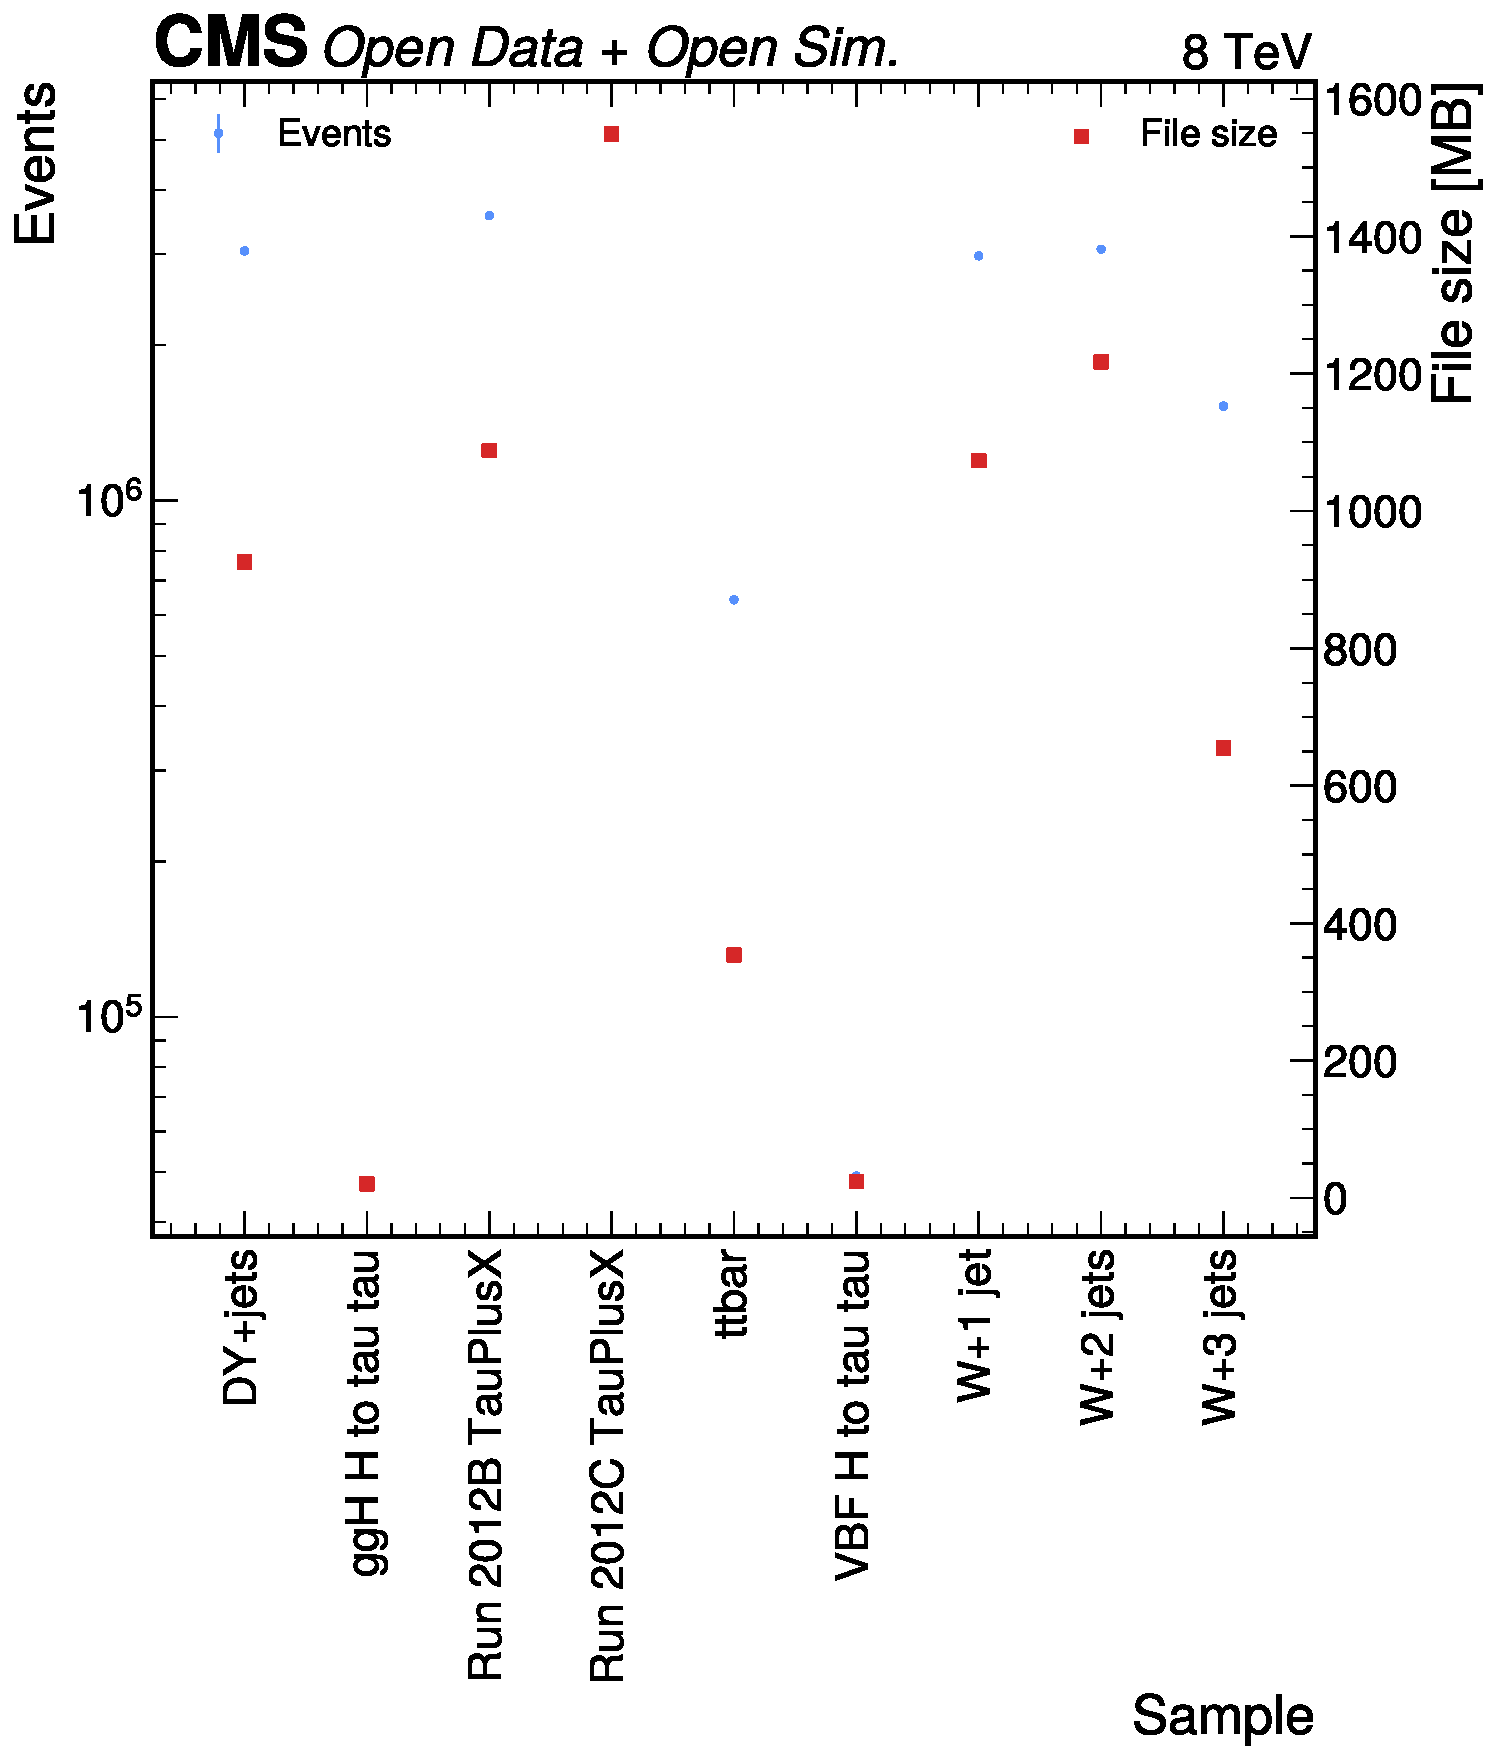
\includegraphics[height=0.35\textheight,width=\linewidth,keepaspectratio,alt={Sample inventory summary. This figure summarizes the localized reduced sample inventory and file-size scale used in the analysis. It documents the available data/MC inputs and shows why the final result is framed as a reduced Open Data search rather than a reproduction of the full CMS publication.}]{figures/sample_event_count_file_size.pdf}}
\caption{Sample inventory summary. This figure summarizes the localized
reduced sample inventory and file-size scale used in the analysis. It
documents the available data/MC inputs and shows why the final result is
framed as a reduced Open Data search rather than a reproduction of the
full CMS publication.}\label{fig:sample-inventory}
\end{figure}

\needspace{4\baselineskip}
\FloatBarrier
\section{Event Selection and
Categories}\label{event-selection-and-categories}

Events are selected using the TauPlusX trigger
\texttt{HLT\_IsoMu17\_eta2p1\_LooseIsoPFTau20}. Muon candidates require
\(p_T > 20\) GeV, \(|\eta| < 2.1\), a tight muon ID, and relative
isolation below 0.20. Hadronic tau candidates require \(p_T > 20\) GeV,
\(|\eta| < 2.3\), decay-mode ID, tight tau isolation ID, tight anti-muon
ID, finite relative isolation, and \(\Delta R(\mu,\tau_h) > 0.5\).

Signal-region candidates are opposite-sign muon-tau pairs with
transverse mass \(m_T(\mu,E_T^{\mathrm{miss}}) < 40\) GeV. The W control
region uses opposite-sign pairs with \(m_T > 80\) GeV. Same-sign
low-\(m_T\) candidates define the reducible-background sideband. A
Z-rich validation region is retained for visible-mass shape checks with
\(60 < m_{\mathrm{vis}} < 120\) GeV.

The transverse mass is

\begin{equation}\protect\phantomsection\label{eq:mt}{
m_T = \sqrt{2 p_T^\mu E_T^{\mathrm{miss}} \left[1-\cos\Delta\phi(\mu,E_T^{\mathrm{miss}})\right]}.
}\end{equation}

Selected events are assigned to mutually exclusive categories. VBF
events are selected first with at least two clean jets and VBF-like
dijet kinematics. Remaining events with at least one clean jet enter the
boosted category. Events without selected jets enter the zero-jet
category. This category order preserves the VBF topology while keeping
the statistical model a simple simultaneous template fit.

{\def\LTcaptype{none} % do not increment counter
\vspace{1em}
\begin{table}[htbp]
\centering
\small
\begin{tabular}{@{}
>{\raggedright\arraybackslash}p{(\linewidth - 2\tabcolsep) * \real{0.5000}}
  >{\raggedright\arraybackslash}p{(\linewidth - 2\tabcolsep) * \real{0.5000}}@{}}
\toprule\noalign{}
\begin{minipage}[b]{\linewidth}\raggedright
Requirement
\end{minipage} & \begin{minipage}[b]{\linewidth}\raggedright
Role in analysis
\end{minipage} \\
\midrule\noalign{}
TauPlusX trigger & Defines the public muon-tau trigger phase space \\
Tight muon and tau IDs & Select prompt muon plus hadronic tau
candidates \\
Tight anti-muon tau ID & Reduces muon fake contamination in the tau\_h
leg \\
Opposite-sign charge & Signal-region charge requirement \\
\(m_T < 40\) GeV & Suppresses W+jets in the signal region \\
VBF / boosted / zero-jet categories & Separate signal-enriched and
control-like event topologies \\
\end{tabular}
\end{table}
}

\needspace{0.4\textheight}
\begin{figure}[htbp]
\centering
\pandocbounded{
\includegraphics[height=0.35\textheight,width=\linewidth,keepaspectratio,alt={Cutflow summary. The cutflow shows raw event counts after each selection step for data, signal MC, and background MC. The monotonic behavior confirms that the final candidate set is produced by cumulative event-selection requirements rather than by a post-fit normalization adjustment.}]{figures/cutflow_summary.pdf}}
\caption{Cutflow summary. The cutflow shows raw event counts after each
selection step for data, signal MC, and background MC. The monotonic
behavior confirms that the final candidate set is produced by cumulative
event-selection requirements rather than by a post-fit normalization
adjustment.}\label{fig:cutflow}
\end{figure}

\needspace{0.4\textheight}
\begin{figure}[htbp]
\centering
\pandocbounded{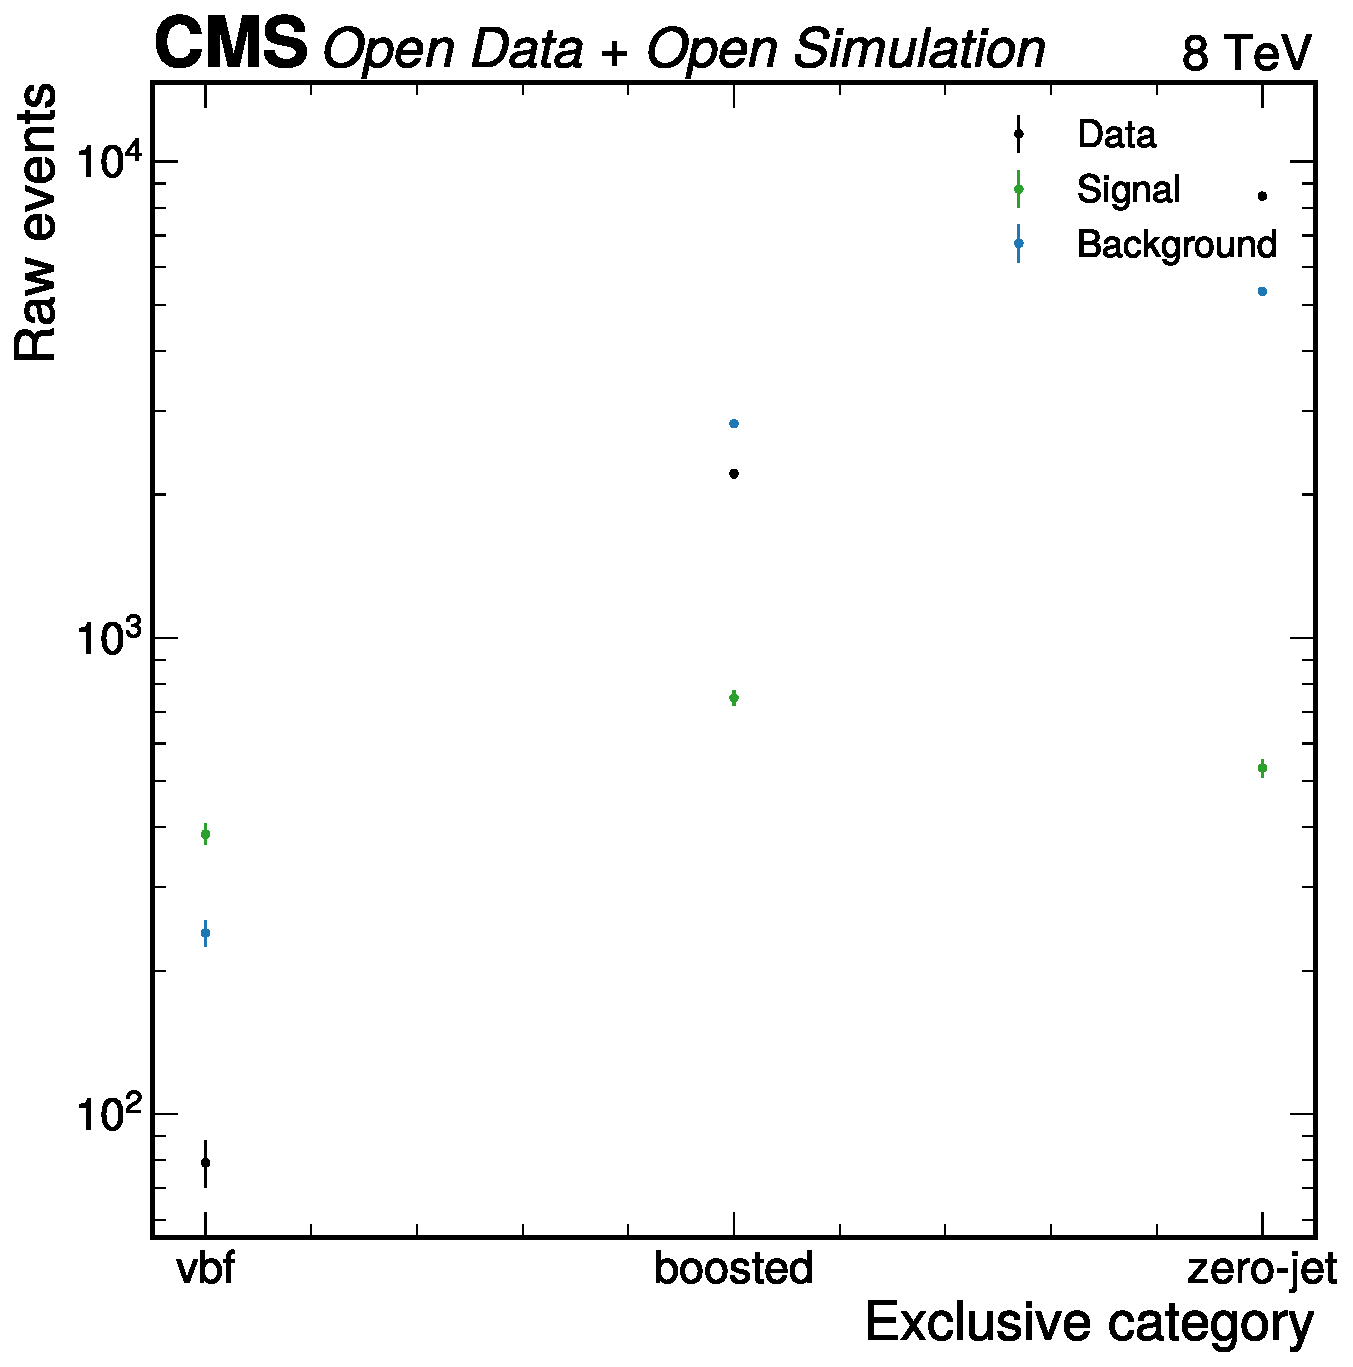
\includegraphics[height=0.35\textheight,width=\linewidth,keepaspectratio,alt={Category yield overview. The category-yield diagnostic shows the VBF, boosted, and zero-jet populations after the signal-region selection. The zero-jet category dominates the statistics, while VBF carries the most topology-specific signal motivation and the largest residual local validation tension.}]{figures/category_yields.pdf}}
\caption{Category yield overview. The category-yield diagnostic shows
the VBF, boosted, and zero-jet populations after the signal-region
selection. The zero-jet category dominates the statistics, while VBF
carries the most topology-specific signal motivation and the largest
residual local validation tension.}\label{fig:category-yields}
\end{figure}

\needspace{4\baselineskip}
\FloatBarrier
\section{Observable Choice and Analysis
Decision}\label{observable-choice-and-analysis-decision}

The final observable is the visible mass \(m_{\mathrm{vis}}\) of the
selected muon and hadronic tau candidate. It is less sensitive than the
optimized classifier in expected-only studies, but it passes the
full-data validation gate in the baseline workspace. The final result
therefore follows the binding strategy that alternatives may replace
visible mass only after validation.

The visible mass is defined from the reconstructed lepton four-vectors
as

\begin{equation}\protect\phantomsection\label{eq:mvis}{
m_{\mathrm{vis}}^2 = \left(p_\mu + p_{\tau_h}\right)^2.
}\end{equation}

The optimized classifier is not a final result. It is documented in
Section~\ref{sec:rejected-classifier} because its observed fit gives a
boundary-like limit, a large fitted signal strength, and a gross
combined data/background mismatch. Keeping it as a rejected diagnostic
preserves the methodological lesson without allowing a failed validation
gate to enter the headline physics result.

\needspace{0.4\textheight}
\begin{figure}[htbp]
\centering
\pandocbounded{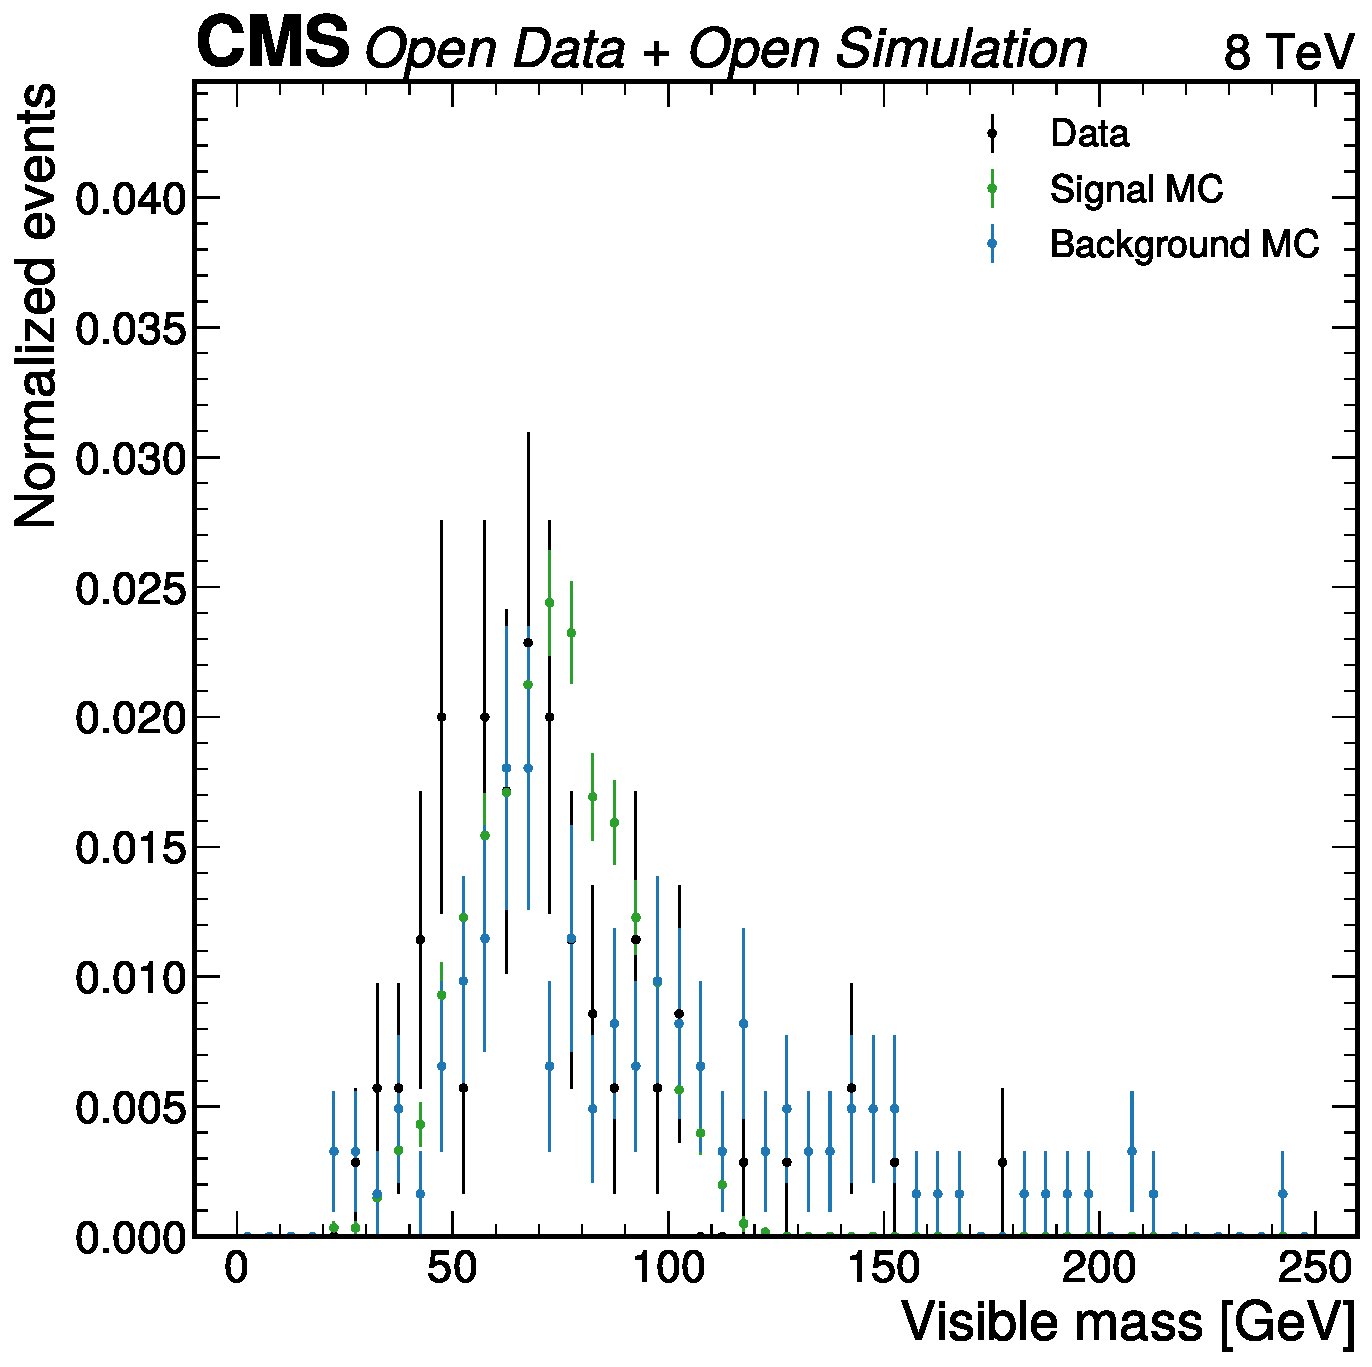
\includegraphics[height=0.35\textheight,width=\linewidth,keepaspectratio,alt={Visible-mass distribution in the VBF category. This pre-fit comparison illustrates the observable used by the final workspace in the VBF topology. The final validation plot in fig.~ adds the exact baseline QCD/fake treatment and category-level validation metrics.}]{figures/visible_mass_vbf.pdf}}
\caption{Visible-mass distribution in the VBF category. This pre-fit
comparison illustrates the observable used by the final workspace in the
VBF topology. The final validation plot in
Figure~\ref{fig:baseline-visible-vbf} adds the exact baseline QCD/fake
treatment and category-level validation
metrics.}\label{fig:phase3-visible-vbf}
\end{figure}

\needspace{0.4\textheight}
\begin{figure}[htbp]
\centering
\pandocbounded{
\includegraphics[height=0.35\textheight,width=\linewidth,keepaspectratio,alt={Visible-mass distribution in the boosted category. This comparison shows that the visible-mass observable retains broad data/MC shape information without relying on the high-score tail that failed for the classifier model. It supports the choice of a robust baseline over the rejected optimization attempt.}]{figures/visible_mass_boosted.pdf}}
\caption{Visible-mass distribution in the boosted category. This
comparison shows that the visible-mass observable retains broad data/MC
shape information without relying on the high-score tail that failed for
the classifier model. It supports the choice of a robust baseline over
the rejected optimization attempt.}\label{fig:phase3-visible-boosted}
\end{figure}

\needspace{0.4\textheight}
\begin{figure}[htbp]
\centering
\pandocbounded{
\includegraphics[height=0.35\textheight,width=\linewidth,keepaspectratio,alt={Visible-mass distribution in the zero-jet category. The zero-jet category provides most of the event count and therefore dominates the global normalization behavior. The final limit remains weak because the visible-mass signal-to-background separation is modest in this category.}]{figures/visible_mass_zero_jet.pdf}}
\caption{Visible-mass distribution in the zero-jet category. The
zero-jet category provides most of the event count and therefore
dominates the global normalization behavior. The final limit remains
weak because the visible-mass signal-to-background separation is modest
in this category.}\label{fig:phase3-visible-zero}
\end{figure}

\needspace{4\baselineskip}
\FloatBarrier
\section{Background Corrections}\label{background-corrections}

The final model uses MC shapes for signal, DY/Z, ttbar, and W+jets, with
data-driven corrections for W+jets normalization, the VBF-background
normalization, and reducible QCD/fake contamination. The control-region
corrections are derived outside the signal fit and then propagated into
the baseline workspace.

The W+jets scale factor is

\begin{equation}\protect\phantomsection\label{eq:w-scale}{
S_W = \frac{N_{\mathrm{data},\mathrm{CR}} - N_{\mathrm{nonW},\mathrm{CR}}}
{N_{W,\mathrm{CR}}},
}\end{equation}

which gives \(S_W = 0.8528 \pm 0.0370\) using 4023 high-\(m_T\) data
events, \(N_W = 2414.78\), and \(N_{\mathrm{nonW}} = 1963.57\). The
relative uncertainty is 4.34\% and is implemented as
\texttt{wjets\_high\_mt\_control}.

The VBF background scale is

\begin{equation}\protect\phantomsection\label{eq:vbf-scale}{
S_{\mathrm{VBF,bkg}} =
\frac{N_{\mathrm{data},\mathrm{VBFCR}}}
{N_{\mathrm{MC,bkg},\mathrm{VBFCR}}},
}\end{equation}

giving \(S_{\mathrm{VBF,bkg}} = 0.5571 \pm 0.0515\). It is applied only
to MC backgrounds in the VBF fit category and is constrained by the
9.24\% \texttt{vbf\_background\_control} nuisance.

The reducible QCD/fake estimate starts from same-sign low-\(m_T\) data
after non-QCD subtraction:

\begin{equation}\protect\phantomsection\label{eq:qcd-transfer}{
N^{\mathrm{QCD}}_{\mathrm{SS},b} = N^{\mathrm{data}}_{\mathrm{SS},b} -
N^{\mathrm{nonQCD}}_{\mathrm{SS},b},
\qquad
N^{\mathrm{QCD}}_{\mathrm{OS},b} = R_{\mathrm{OS/SS}} N^{\mathrm{QCD}}_{\mathrm{SS},b}.
}\end{equation}

For the final baseline workspace the retained transfer-factor nuisance
is 12.060\%. The current artifact records a limitation: QCD
shape-statistical uncertainties are included in validation variances but
are not expanded into per-bin pyhf nuisances in the baseline workspace.
This is a documented limitation of the reduced analysis rather than a
hidden source of sensitivity.

{\def\LTcaptype{none} % do not increment counter
\vspace{1em}
\begin{table}[htbp]
\centering
\small
\begin{tabular}{@{}
>{\raggedright\arraybackslash}p{(\linewidth - 6\tabcolsep) * \real{0.2308}}
  >{\raggedright\arraybackslash}p{(\linewidth - 6\tabcolsep) * \real{0.2308}}
  >{\raggedleft\arraybackslash}p{(\linewidth - 6\tabcolsep) * \real{0.3077}}
  >{\raggedright\arraybackslash}p{(\linewidth - 6\tabcolsep) * \real{0.2308}}@{}}
\toprule\noalign{}
\begin{minipage}[b]{\linewidth}\raggedright
Control input
\end{minipage} & \begin{minipage}[b]{\linewidth}\raggedright
Formula
\end{minipage} & \begin{minipage}[b]{\linewidth}\raggedleft
Value
\end{minipage} & \begin{minipage}[b]{\linewidth}\raggedright
Use in final model
\end{minipage} \\
\midrule\noalign{}
W high-\(m_T\) scale & Equation~\ref{eq:w-scale} & 0.8528 ± 0.0370 & W+jets
normalization nuisance \\
VBF background scale & Equation~\ref{eq:vbf-scale} & 0.5571 ± 0.0515 & VBF
MC-background nuisance \\
Same-sign QCD/fake transfer & Equation~\ref{eq:qcd-transfer} & 12.060\%
relative uncertainty & Global QCD/fake transfer nuisance \\
\end{tabular}
\end{table}
}

\needspace{0.4\textheight}
\begin{figure}[htbp]
\centering
\pandocbounded{
\includegraphics[height=0.35\textheight,width=\linewidth,keepaspectratio,alt={QCD same-sign visible-mass control. This figure shows the same-sign sideband used to form the reducible-background template. The final note treats the transfer-factor limitations explicitly because the reduced Open Data format does not provide an anti-isolated tau branch for a fuller fake-factor method.}]{figures/qcd_same_sign_mvis.pdf}}
\caption{QCD same-sign visible-mass control. This figure shows the
same-sign sideband used to form the reducible-background template. The
final note treats the transfer-factor limitations explicitly because the
reduced Open Data format does not provide an anti-isolated tau branch
for a fuller fake-factor method.}\label{fig:qcd-ss}
\end{figure}

\needspace{4\baselineskip}
\FloatBarrier
\section{Statistical Model}\label{statistical-model}

The final result uses a binned pyhf/HistFactory likelihood (Heinrich et
al. 2021). For category \(c\) and visible-mass bin \(b\), the expected
yield is

\begin{equation}\protect\phantomsection\label{eq:bin-yield}{
\lambda_{cb}(\mu,\boldsymbol{\theta}) =
\mu s_{cb}(\boldsymbol{\theta}) +
\sum_k b_{kcb}(\boldsymbol{\theta}) +
q_{cb}(\boldsymbol{\theta}),
}\end{equation}

where \(s\) is the combined ggH and VBF Higgs signal, \(b_k\) are
simulation-derived backgrounds, and \(q\) is the same-sign data-driven
QCD/fake template. The likelihood is

\begin{equation}\protect\phantomsection\label{eq:likelihood}{
L(\mu,\boldsymbol{\theta}) =
\prod_{c,b} \mathrm{Pois}\left(n_{cb}\mid \lambda_{cb}(\mu,\boldsymbol{\theta})\right)
\prod_j \pi_j(\theta_j),
}\end{equation}

with Gaussian/log-normal constrained nuisance parameters and staterror
terms for finite MC precision. The fit constrains \(\mu \ge 0\).

Upper limits use the modified frequentist CLs construction (Read 2002):

\begin{equation}\protect\phantomsection\label{eq:cls}{
\mathrm{CL}_s(\mu)=\frac{p_{s+b}(q_\mu \ge q_\mu^{\mathrm{obs}})}
{p_b(q_\mu \ge q_\mu^{\mathrm{obs}})}.
}\end{equation}

The quoted 95\% limit is the value of \(\mu\) where
\(\mathrm{CL}_s=0.05\). The profile interval printed for the best fit
solves

\begin{equation}\protect\phantomsection\label{eq:profile-interval}{
q(\mu)= -2\ln\frac{L(\mu,\hat{\boldsymbol{\theta}}_\mu)}
{L(\hat{\mu},\hat{\boldsymbol{\theta}})} = 1,
}\end{equation}

with the lower side bounded at \(\mu=0\) when required. Asymptotic
formulae are used for the reported limits and diagnostics (Cowan et al.
2011). The final bins all have enough total expected background for an
initial asymptotic interpretation, but no full observed-data toy
ensemble is stored in the current Phase 5 artifacts; this remains an
explicit limitation.

\needspace{4\baselineskip}
\FloatBarrier
\section{Systematic Uncertainties}\label{systematic-uncertainties}

The final systematic program follows the search-convention categories
that are implementable with the reduced inputs: luminosity,
object/acceptance, DY/Z normalization, W control, VBF control, QCD/fake
transfer, and MC statistical uncertainty. Missing full-analysis
components are documented as limitations rather than replaced by
arbitrary uncertainty inflation.

{\def\LTcaptype{none} % do not increment counter
\vspace{1em}
\begin{table}[htbp]
\centering
\small
\begin{tabular}{@{}
>{\raggedright\arraybackslash}p{(\linewidth - 6\tabcolsep) * \real{0.2308}}
  >{\raggedleft\arraybackslash}p{(\linewidth - 6\tabcolsep) * \real{0.3077}}
  >{\raggedright\arraybackslash}p{(\linewidth - 6\tabcolsep) * \real{0.2308}}
  >{\raggedright\arraybackslash}p{(\linewidth - 6\tabcolsep) * \real{0.2308}}@{}}
\toprule\noalign{}
\begin{minipage}[b]{\linewidth}\raggedright
Source
\end{minipage} & \begin{minipage}[b]{\linewidth}\raggedleft
Value
\end{minipage} & \begin{minipage}[b]{\linewidth}\raggedright
Scope
\end{minipage} & \begin{minipage}[b]{\linewidth}\raggedright
Motivation
\end{minipage} \\
\midrule\noalign{}
Luminosity & 2.6\% & All simulation-normalized signal and background
samples & CMS 2012 luminosity normalization used by the Open Data
records \\
Tau/open-data acceptance & 15\% & Signal and MC backgrounds selected
with the reduced muon-tau objects & Open Data reduced-sample acceptance
and missing public trigger/tau scale-factor coverage \\
DY/Z normalization & 15\% & DYJetsToLL in all visible-mass categories &
Reduced-sample DY/Z validation and missing embedded/electroweak Z
components \\
W high-mT control & 4.344\% & W1JetsToLNu, W2JetsToLNu, W3JetsToLNu &
Full-data high-mT control-region scale factor \\
VBF background control & 9.237\% & MC backgrounds in the VBF category &
VBF-like top-btag non-signal control region \\
Same-sign QCD/fake transfer & 12.060\% & Data-driven QCD/fake template
in all baseline categories & Same-sign low-mT sideband transfer factor
retained by the baseline workspace \\
MC statistical uncertainty & per-bin sumw2 & Every MC-filled bin in each
category & Finite reduced MC counts and official Open Data normalization
weights \\
\end{tabular}
\end{table}
}

\needspace{0.4\textheight}
\begin{figure}[htbp]
\centering
\pandocbounded{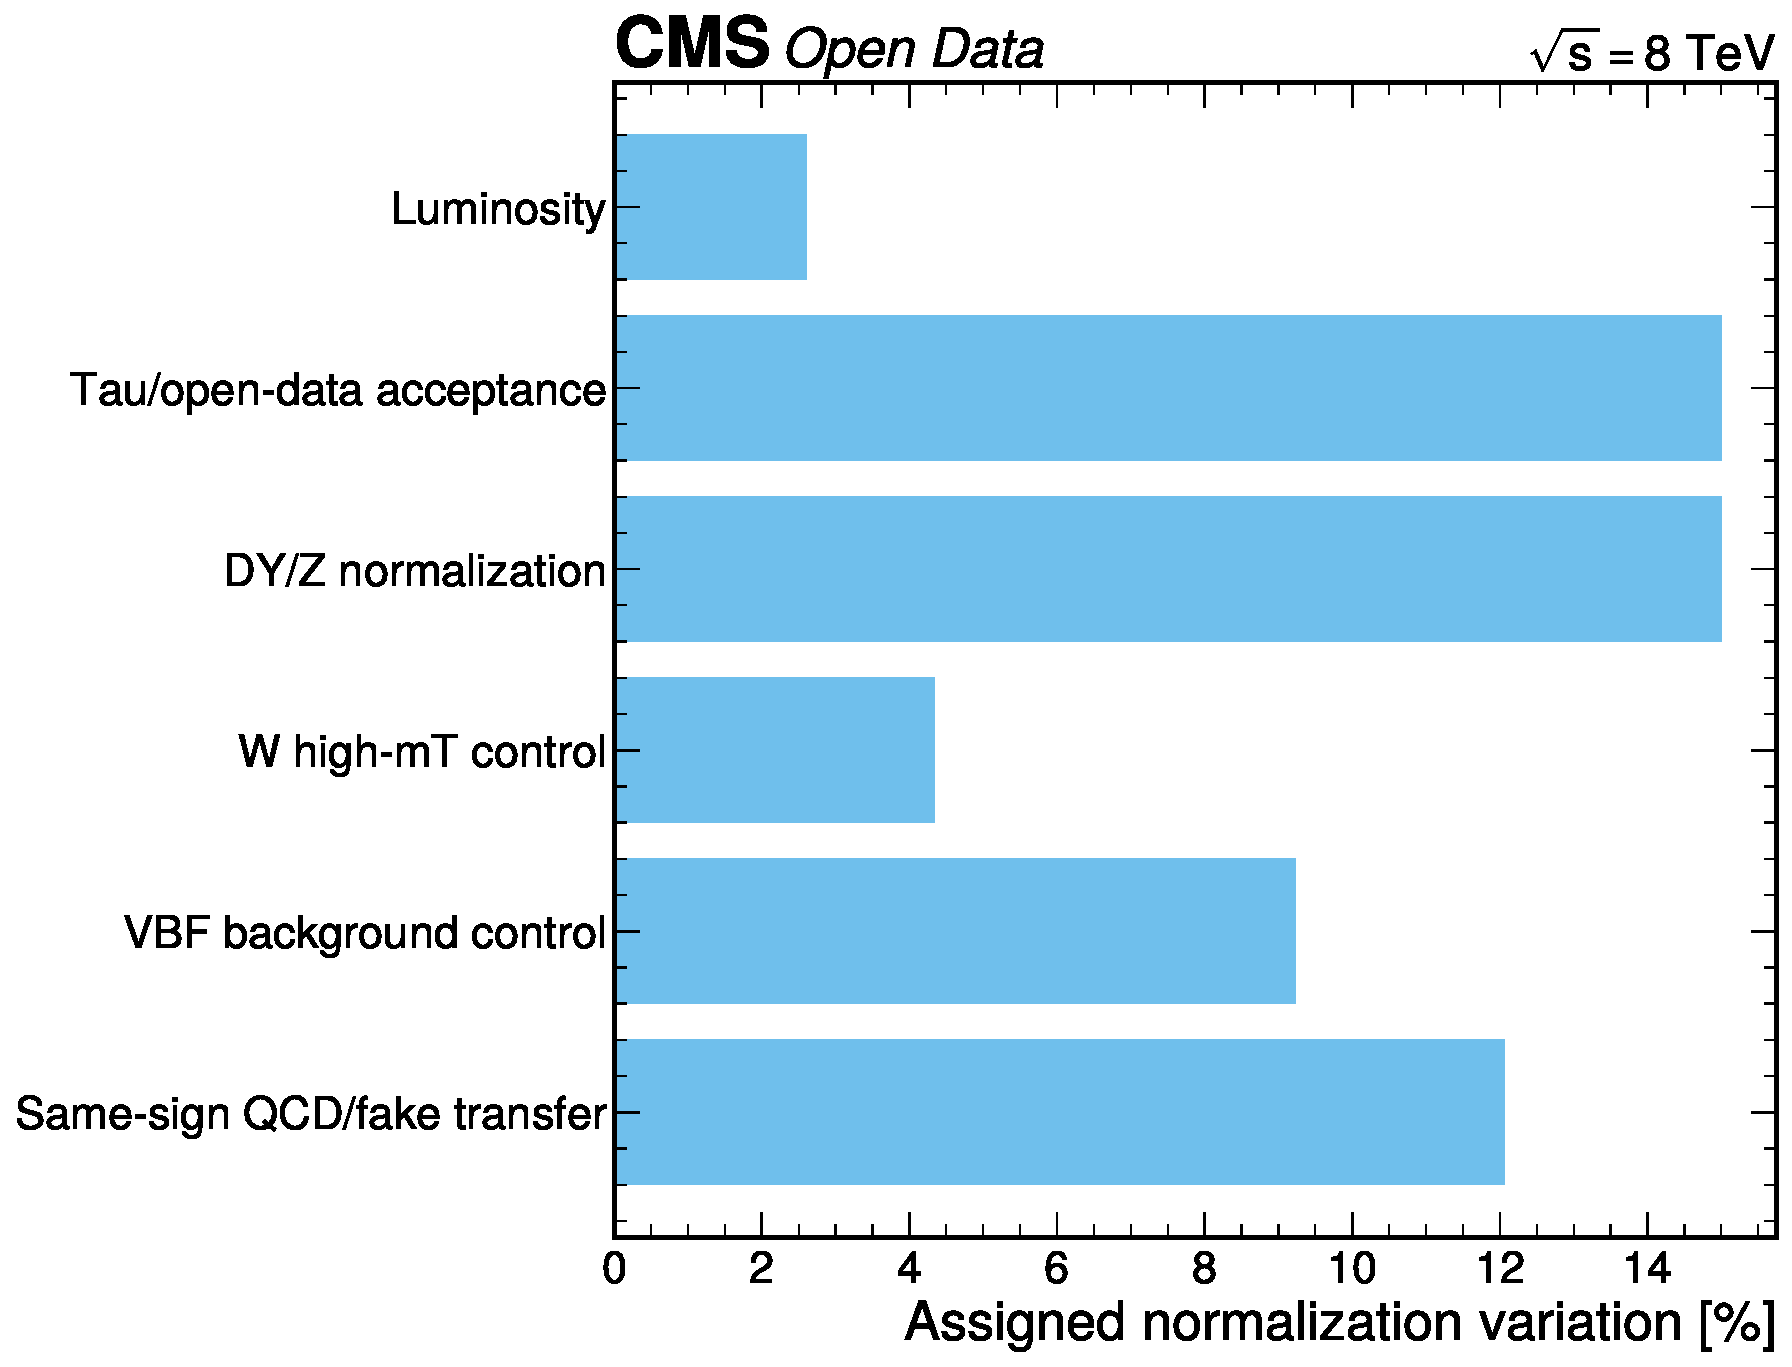
\includegraphics[height=0.35\textheight,width=\linewidth,keepaspectratio,alt={Baseline systematic program. The figure summarizes the assigned normalization variations implemented in the final visible-mass workspace. It is not an impact ranking; exact source-by-source impacts are not available in the current JSON outputs and are therefore not fabricated.}]{figures/phase5_systematic_program_baseline.pdf}}
\caption{Baseline systematic program. The figure summarizes the assigned
normalization variations implemented in the final visible-mass
workspace. It is not an impact ranking; exact source-by-source impacts
are not available in the current JSON outputs and are therefore not
fabricated.}\label{fig:systematic-program}
\end{figure}

\needspace{4\baselineskip}
\subsection{Luminosity}\label{luminosity}

Physical origin: CMS 2012 luminosity normalization used by the Open Data
records. The source is retained because it changes either the absolute
MC normalization, the transfer of a data-driven background into the
signal region, or the bin-by-bin template precision used by the
likelihood.

Evaluation method: the baseline pyhf workspace implements
\texttt{lumi\_2012} with value 2.6\% for All simulation-normalized
signal and background samples. The correlation model is: One nuisance
correlated across categories and MC samples. For normalization
systematics the nuisance multiplies the affected yields through
log-normal interpolation,

\begin{equation}\protect\phantomsection\label{eq:normsys-lumi-2012}{
\nu_{p}(\theta_p)=
\begin{cases}
\nu^0_p\,\kappa_{p,+}^{\theta_p}, & \theta_p \ge 0, \\
\nu^0_p\,\kappa_{p,-}^{-\theta_p}, & \theta_p < 0,
\end{cases}
}\end{equation}

where \(\nu^0_p\) is the nominal bin yield and \(\theta_p\) is
constrained by a unit Gaussian. MC statistical terms use the per-bin
staterror modifiers stored in
\texttt{pyhf\_workspace\_baseline\_visible.json}.

Numerical impact: Included in the baseline workspace. A standalone
impact ranking is not available in the current JSON artifacts. The final
artifact does not store a source-by-source refit impact on \texttt{mu};
the note therefore reports the implemented nuisance value, affected
samples, fitted nuisance value when applicable, and an explicit
limitation rather than fabricating an impact ranking.

Interpretation: this source is part of the final error model used for
the CLs limit. Its adequacy is judged together with the visible-mass
validation plots, nuisance-pull summary, and the low-sensitivity result
interpretation.

\needspace{4\baselineskip}
\subsection{Tau/open-data acceptance}\label{tauopen-data-acceptance}

Physical origin: Open Data reduced-sample acceptance and missing public
trigger/tau scale-factor coverage. The source is retained because it
changes either the absolute MC normalization, the transfer of a
data-driven background into the signal region, or the bin-by-bin
template precision used by the likelihood.

Evaluation method: the baseline pyhf workspace implements
\texttt{tau\_open\_data\_acceptance} with value 15\% for Signal and MC
backgrounds selected with the reduced muon-tau objects. The correlation
model is: One nuisance correlated across categories and MC samples. For
normalization systematics the nuisance multiplies the affected yields
through log-normal interpolation,

\begin{equation}\protect\phantomsection\label{eq:normsys-tau-open-data-acceptance}{
\nu_{p}(\theta_p)=
\begin{cases}
\nu^0_p\,\kappa_{p,+}^{\theta_p}, & \theta_p \ge 0, \\
\nu^0_p\,\kappa_{p,-}^{-\theta_p}, & \theta_p < 0,
\end{cases}
}\end{equation}

where \(\nu^0_p\) is the nominal bin yield and \(\theta_p\) is
constrained by a unit Gaussian. MC statistical terms use the per-bin
staterror modifiers stored in
\texttt{pyhf\_workspace\_baseline\_visible.json}.

Numerical impact: Included in the baseline workspace. The fitted pull is
reported; per-source mu impact is not stored. The final artifact does
not store a source-by-source refit impact on \texttt{mu}; the note
therefore reports the implemented nuisance value, affected samples,
fitted nuisance value when applicable, and an explicit limitation rather
than fabricating an impact ranking.

Interpretation: this source is part of the final error model used for
the CLs limit. Its adequacy is judged together with the visible-mass
validation plots, nuisance-pull summary, and the low-sensitivity result
interpretation.

\needspace{4\baselineskip}
\subsection{DY/Z normalization}\label{dyz-normalization}

Physical origin: Reduced-sample DY/Z validation and missing
embedded/electroweak Z components. The source is retained because it
changes either the absolute MC normalization, the transfer of a
data-driven background into the signal region, or the bin-by-bin
template precision used by the likelihood.

Evaluation method: the baseline pyhf workspace implements
\texttt{dy\_norm\_open\_data} with value 15\% for DYJetsToLL in all
visible-mass categories. The correlation model is: One nuisance
correlated across categories. For normalization systematics the nuisance
multiplies the affected yields through log-normal interpolation,

\begin{equation}\protect\phantomsection\label{eq:normsys-dy-norm-open-data}{
\nu_{p}(\theta_p)=
\begin{cases}
\nu^0_p\,\kappa_{p,+}^{\theta_p}, & \theta_p \ge 0, \\
\nu^0_p\,\kappa_{p,-}^{-\theta_p}, & \theta_p < 0,
\end{cases}
}\end{equation}

where \(\nu^0_p\) is the nominal bin yield and \(\theta_p\) is
constrained by a unit Gaussian. MC statistical terms use the per-bin
staterror modifiers stored in
\texttt{pyhf\_workspace\_baseline\_visible.json}.

Numerical impact: Included in the baseline workspace. It has the largest
non-MC-stat fitted pull among retained global nuisances. The final
artifact does not store a source-by-source refit impact on \texttt{mu};
the note therefore reports the implemented nuisance value, affected
samples, fitted nuisance value when applicable, and an explicit
limitation rather than fabricating an impact ranking.

Interpretation: this source is part of the final error model used for
the CLs limit. Its adequacy is judged together with the visible-mass
validation plots, nuisance-pull summary, and the low-sensitivity result
interpretation.

\needspace{4\baselineskip}
\subsection{W high-mT control}\label{w-high-mt-control}

Physical origin: Full-data high-mT control-region scale factor. The
source is retained because it changes either the absolute MC
normalization, the transfer of a data-driven background into the signal
region, or the bin-by-bin template precision used by the likelihood.

Evaluation method: the baseline pyhf workspace implements
\texttt{wjets\_high\_mt\_control} with value 4.344\% for W1JetsToLNu,
W2JetsToLNu, W3JetsToLNu. The correlation model is: One nuisance
correlated across W+jets samples and categories. For normalization
systematics the nuisance multiplies the affected yields through
log-normal interpolation,

\begin{equation}\protect\phantomsection\label{eq:normsys-wjets-high-mt-control}{
\nu_{p}(\theta_p)=
\begin{cases}
\nu^0_p\,\kappa_{p,+}^{\theta_p}, & \theta_p \ge 0, \\
\nu^0_p\,\kappa_{p,-}^{-\theta_p}, & \theta_p < 0,
\end{cases}
}\end{equation}

where \(\nu^0_p\) is the nominal bin yield and \(\theta_p\) is
constrained by a unit Gaussian. MC statistical terms use the per-bin
staterror modifiers stored in
\texttt{pyhf\_workspace\_baseline\_visible.json}.

Numerical impact: Included in the baseline workspace. The control-region
derivation is tabulated in the note. The final artifact does not store a
source-by-source refit impact on \texttt{mu}; the note therefore reports
the implemented nuisance value, affected samples, fitted nuisance value
when applicable, and an explicit limitation rather than fabricating an
impact ranking.

Interpretation: this source is part of the final error model used for
the CLs limit. Its adequacy is judged together with the visible-mass
validation plots, nuisance-pull summary, and the low-sensitivity result
interpretation.

\needspace{4\baselineskip}
\subsection{VBF background control}\label{vbf-background-control}

Physical origin: VBF-like top-btag non-signal control region. The source
is retained because it changes either the absolute MC normalization, the
transfer of a data-driven background into the signal region, or the
bin-by-bin template precision used by the likelihood.

Evaluation method: the baseline pyhf workspace implements
\texttt{vbf\_background\_control} with value 9.237\% for MC backgrounds
in the VBF category. The correlation model is: One nuisance applied only
to VBF-category MC backgrounds. For normalization systematics the
nuisance multiplies the affected yields through log-normal
interpolation,

\begin{equation}\protect\phantomsection\label{eq:normsys-vbf-background-control}{
\nu_{p}(\theta_p)=
\begin{cases}
\nu^0_p\,\kappa_{p,+}^{\theta_p}, & \theta_p \ge 0, \\
\nu^0_p\,\kappa_{p,-}^{-\theta_p}, & \theta_p < 0,
\end{cases}
}\end{equation}

where \(\nu^0_p\) is the nominal bin yield and \(\theta_p\) is
constrained by a unit Gaussian. MC statistical terms use the per-bin
staterror modifiers stored in
\texttt{pyhf\_workspace\_baseline\_visible.json}.

Numerical impact: Included in the baseline workspace. Residual VBF
validation tension is discussed separately. The final artifact does not
store a source-by-source refit impact on \texttt{mu}; the note therefore
reports the implemented nuisance value, affected samples, fitted
nuisance value when applicable, and an explicit limitation rather than
fabricating an impact ranking.

Interpretation: this source is part of the final error model used for
the CLs limit. Its adequacy is judged together with the visible-mass
validation plots, nuisance-pull summary, and the low-sensitivity result
interpretation.

\needspace{4\baselineskip}
\subsection{Same-sign QCD/fake
transfer}\label{same-sign-qcdfake-transfer}

Physical origin: Same-sign low-mT sideband transfer factor retained by
the baseline workspace. The source is retained because it changes either
the absolute MC normalization, the transfer of a data-driven background
into the signal region, or the bin-by-bin template precision used by the
likelihood.

Evaluation method: the baseline pyhf workspace implements
\texttt{qcd\_ss\_transfer} with value 12.060\% for Data-driven QCD/fake
template in all baseline categories. The correlation model is: One
global transfer-factor nuisance. For normalization systematics the
nuisance multiplies the affected yields through log-normal
interpolation,

\begin{equation}\protect\phantomsection\label{eq:normsys-qcd-ss-transfer}{
\nu_{p}(\theta_p)=
\begin{cases}
\nu^0_p\,\kappa_{p,+}^{\theta_p}, & \theta_p \ge 0, \\
\nu^0_p\,\kappa_{p,-}^{-\theta_p}, & \theta_p < 0,
\end{cases}
}\end{equation}

where \(\nu^0_p\) is the nominal bin yield and \(\theta_p\) is
constrained by a unit Gaussian. MC statistical terms use the per-bin
staterror modifiers stored in
\texttt{pyhf\_workspace\_baseline\_visible.json}.

Numerical impact: Included in the baseline workspace. Shape-statistical
QCD uncertainties are recorded for validation but not expanded into
per-bin pyhf nuisances. The final artifact does not store a
source-by-source refit impact on \texttt{mu}; the note therefore reports
the implemented nuisance value, affected samples, fitted nuisance value
when applicable, and an explicit limitation rather than fabricating an
impact ranking.

Interpretation: this source is part of the final error model used for
the CLs limit. Its adequacy is judged together with the visible-mass
validation plots, nuisance-pull summary, and the low-sensitivity result
interpretation.

\needspace{4\baselineskip}
\subsection{MC statistical
uncertainty}\label{mc-statistical-uncertainty}

Physical origin: Finite reduced MC counts and official Open Data
normalization weights. The source is retained because it changes either
the absolute MC normalization, the transfer of a data-driven background
into the signal region, or the bin-by-bin template precision used by the
likelihood.

Evaluation method: the baseline pyhf workspace implements
\texttt{mc\_stat\_*} with value per-bin sumw2 for Every MC-filled bin in
each category. The correlation model is: Independent Barlow-Beeston-lite
staterror terms by category/bin. For normalization systematics the
nuisance multiplies the affected yields through log-normal
interpolation,

\begin{equation}\protect\phantomsection\label{eq:normsys-mc-stat-stat}{
\nu_{p}(\theta_p)=
\begin{cases}
\nu^0_p\,\kappa_{p,+}^{\theta_p}, & \theta_p \ge 0, \\
\nu^0_p\,\kappa_{p,-}^{-\theta_p}, & \theta_p < 0,
\end{cases}
}\end{equation}

where \(\nu^0_p\) is the nominal bin yield and \(\theta_p\) is
constrained by a unit Gaussian. MC statistical terms use the per-bin
staterror modifiers stored in
\texttt{pyhf\_workspace\_baseline\_visible.json}.

Numerical impact: Included in the baseline workspace. Individual bin
pulls are listed in the nuisance appendix. The final artifact does not
store a source-by-source refit impact on \texttt{mu}; the note therefore
reports the implemented nuisance value, affected samples, fitted
nuisance value when applicable, and an explicit limitation rather than
fabricating an impact ranking.

Interpretation: this source is part of the final error model used for
the CLs limit. Its adequacy is judged together with the visible-mass
validation plots, nuisance-pull summary, and the low-sensitivity result
interpretation.

The error-budget narrative is therefore qualitative but artifact-backed.
The observed interval is dominated by the weak visible-mass separation
and broad allowed nuisance movement, not by a single documented source
exceeding 80\% of the total uncertainty. The current machine outputs do
not store source-by-source impact refits, so a quantitative dominance
claim would be unjustified. A future extension should run a
nuisance-impact scan for the final baseline workspace and store the
resulting \texttt{mu} shifts in JSON.

\needspace{4\baselineskip}
\FloatBarrier
\section{Baseline Validation}\label{baseline-validation}

The visible-mass final result passes the configured full-data validation
gate. Combined over categories, the baseline has data/background =
0.9812, chi2/ndf = 0.7224, and no category or combined validation flag.
The zero-jet chi2/ndf is low at 0.113; this is not algebraically zero,
but it is noted as possible overcoverage from conservative diagonal
validation uncertainties.

{\def\LTcaptype{none} % do not increment counter
\vspace{1em}
\begin{table}[htbp]
\centering
\small
\begin{tabular}{@{}
>{\raggedright\arraybackslash}p{(\linewidth - 14\tabcolsep) * \real{0.0968}}
  >{\raggedleft\arraybackslash}p{(\linewidth - 14\tabcolsep) * \real{0.1290}}
  >{\raggedleft\arraybackslash}p{(\linewidth - 14\tabcolsep) * \real{0.1290}}
  >{\raggedleft\arraybackslash}p{(\linewidth - 14\tabcolsep) * \real{0.1290}}
  >{\raggedleft\arraybackslash}p{(\linewidth - 14\tabcolsep) * \real{0.1290}}
  >{\raggedleft\arraybackslash}p{(\linewidth - 14\tabcolsep) * \real{0.1290}}
  >{\raggedleft\arraybackslash}p{(\linewidth - 14\tabcolsep) * \real{0.1290}}
  >{\raggedleft\arraybackslash}p{(\linewidth - 14\tabcolsep) * \real{0.1290}}@{}}
\toprule\noalign{}
\begin{minipage}[b]{\linewidth}\raggedright
Category
\end{minipage} & \begin{minipage}[b]{\linewidth}\raggedleft
Data
\end{minipage} & \begin{minipage}[b]{\linewidth}\raggedleft
Background
\end{minipage} & \begin{minipage}[b]{\linewidth}\raggedleft
QCD/fake
\end{minipage} & \begin{minipage}[b]{\linewidth}\raggedleft
Signal
\end{minipage} & \begin{minipage}[b]{\linewidth}\raggedleft
D/B
\end{minipage} & \begin{minipage}[b]{\linewidth}\raggedleft
Chi2/ndf
\end{minipage} & \begin{minipage}[b]{\linewidth}\raggedleft
Max pull
\end{minipage} \\
\midrule\noalign{}
VBF & 78 & 96.28 & 17.75 & 1.590 & 0.810 & 1.449 & 2.66 \\
Boosted & 2183 & 2364.39 & 325.58 & 9.170 & 0.923 & 0.605 & 1.25 \\
Zero-jet & 8451 & 8456.81 & 1569.65 & 14.341 & 0.999 & 0.113 & 0.57 \\
\end{tabular}
\end{table}
}

The VBF category has the largest residual local tension: max
\textbar pull\textbar{} = 2.66 and one bin ratio reaches 0.285. This
does not invalidate the final result because the VBF event count is
small, the combined validation passes, and the final interpretation is a
weak upper limit rather than evidence. It is nevertheless a leading
target for a future analysis with fuller background samples and a richer
VBF validation region.

\needspace{0.4\textheight}
\begin{figure}[htbp]
\centering
\pandocbounded{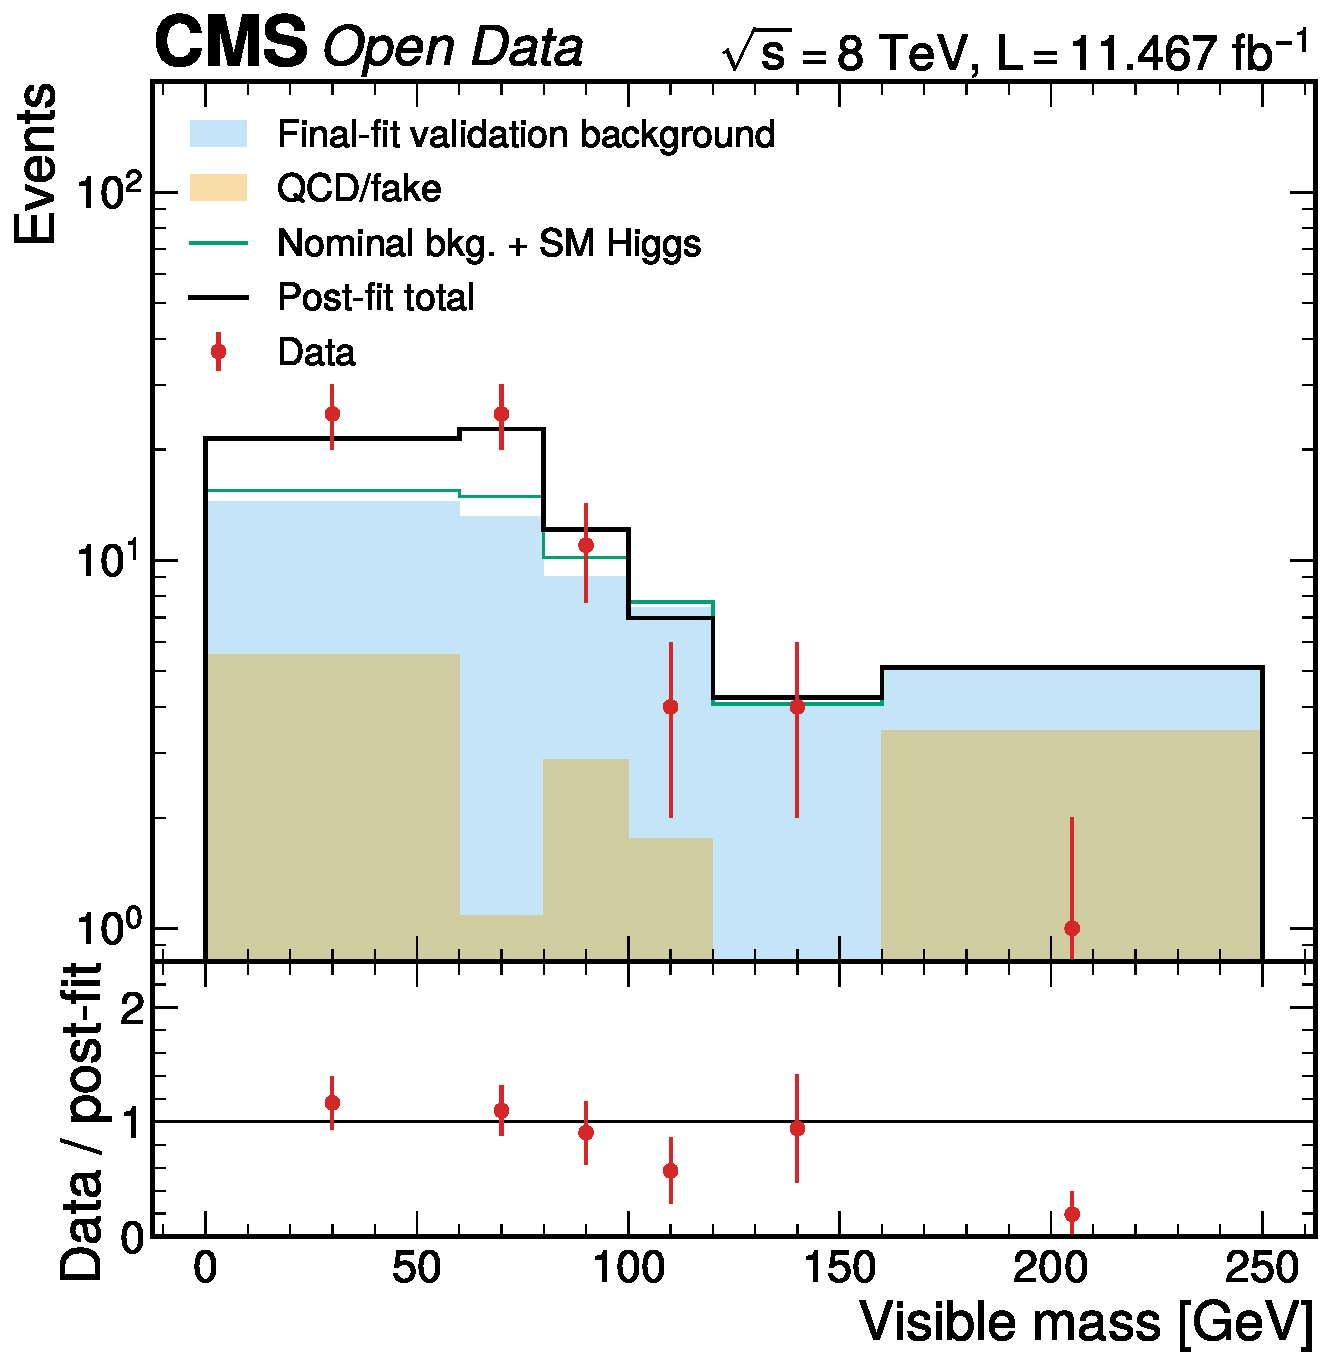
\includegraphics[height=0.35\textheight,width=\linewidth,keepaspectratio,alt={Baseline visible-mass validation in VBF. This regenerated Phase 5 figure compares the final visible-mass model to the full data in the VBF category. The residual local deficit is visible in the ratio panel and is included in the validation summary rather than hidden by the combined pass.}]{figures/phase5_baseline_visible_vbf.pdf}}
\caption{Baseline visible-mass validation in VBF. This regenerated Phase
5 figure compares the final visible-mass model to the full data in the
VBF category. The residual local deficit is visible in the ratio panel
and is included in the validation summary rather than hidden by the
combined pass.}\label{fig:baseline-visible-vbf}
\end{figure}

\needspace{0.4\textheight}
\begin{figure}[htbp]
\centering
\pandocbounded{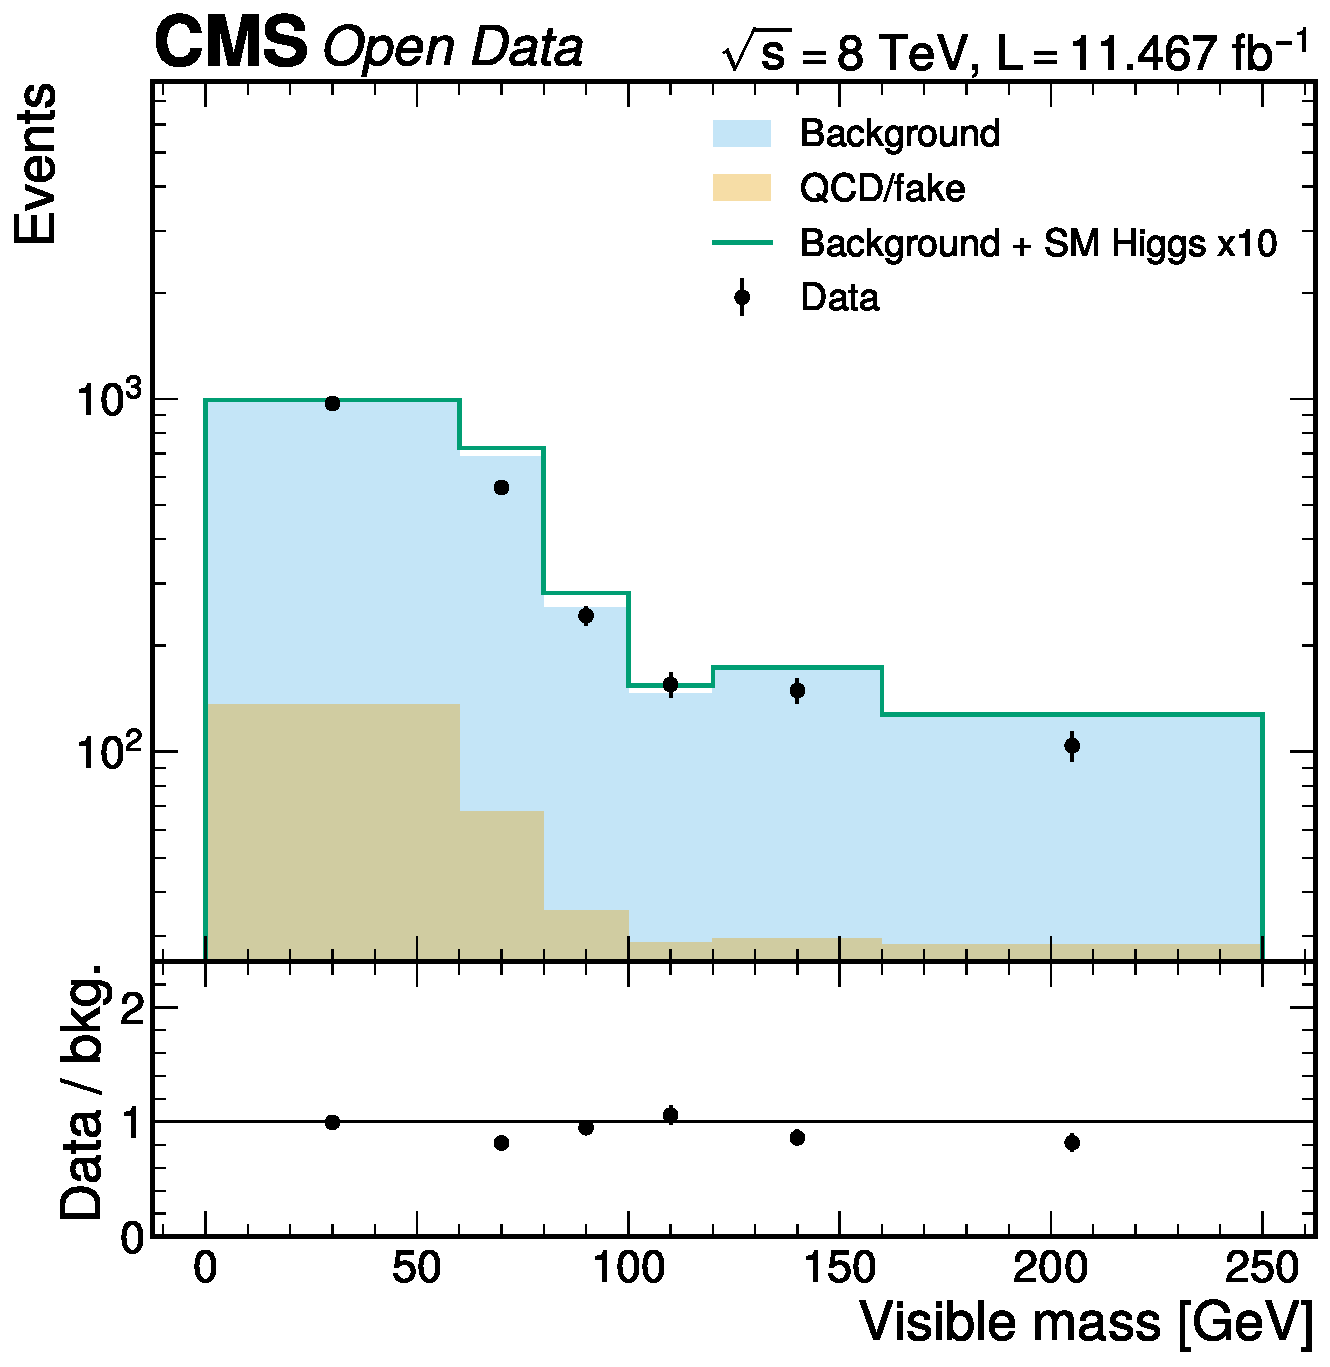
\includegraphics[height=0.35\textheight,width=\linewidth,keepaspectratio,alt={Baseline visible-mass validation in boosted. This regenerated Phase 5 figure shows that the boosted category is globally compatible with the final background model. Its residual pulls are below the VBF maximum and do not drive the final limit.}]{figures/phase5_baseline_visible_boosted.pdf}}
\caption{Baseline visible-mass validation in boosted. This regenerated
Phase 5 figure shows that the boosted category is globally compatible
with the final background model. Its residual pulls are below the VBF
maximum and do not drive the final
limit.}\label{fig:baseline-visible-boosted}
\end{figure}

\needspace{0.4\textheight}
\begin{figure}[htbp]
\centering
\pandocbounded{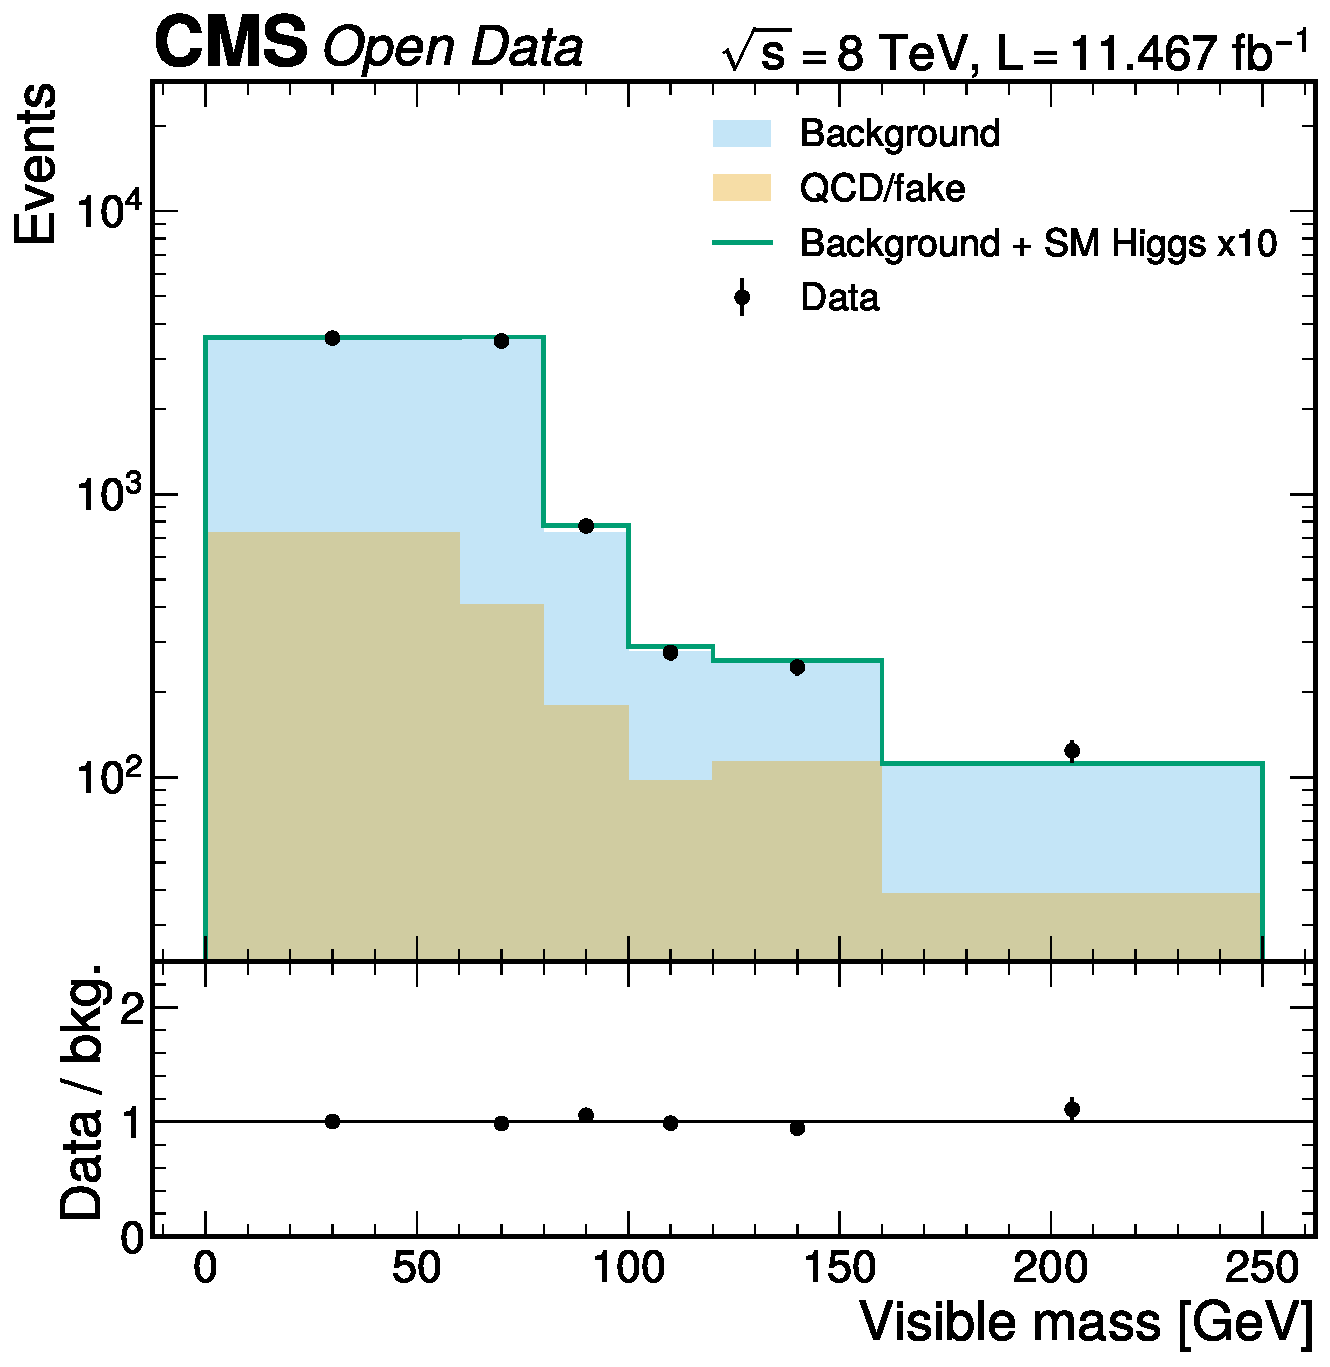
\includegraphics[height=0.35\textheight,width=\linewidth,keepaspectratio,alt={Baseline visible-mass validation in zero-jet. This regenerated Phase 5 figure shows the dominant-statistics zero-jet category for the final result. The ratio panel has no shared-axis text artifact and is the public validation plot used by the final AN.}]{figures/phase5_baseline_visible_zero_jet.pdf}}
\caption{Baseline visible-mass validation in zero-jet. This regenerated
Phase 5 figure shows the dominant-statistics zero-jet category for the
final result. The ratio panel has no shared-axis text artifact and is
the public validation plot used by the final
AN.}\label{fig:baseline-visible-zero}
\end{figure}

\needspace{0.4\textheight}
\begin{figure}[htbp]
\centering
\pandocbounded{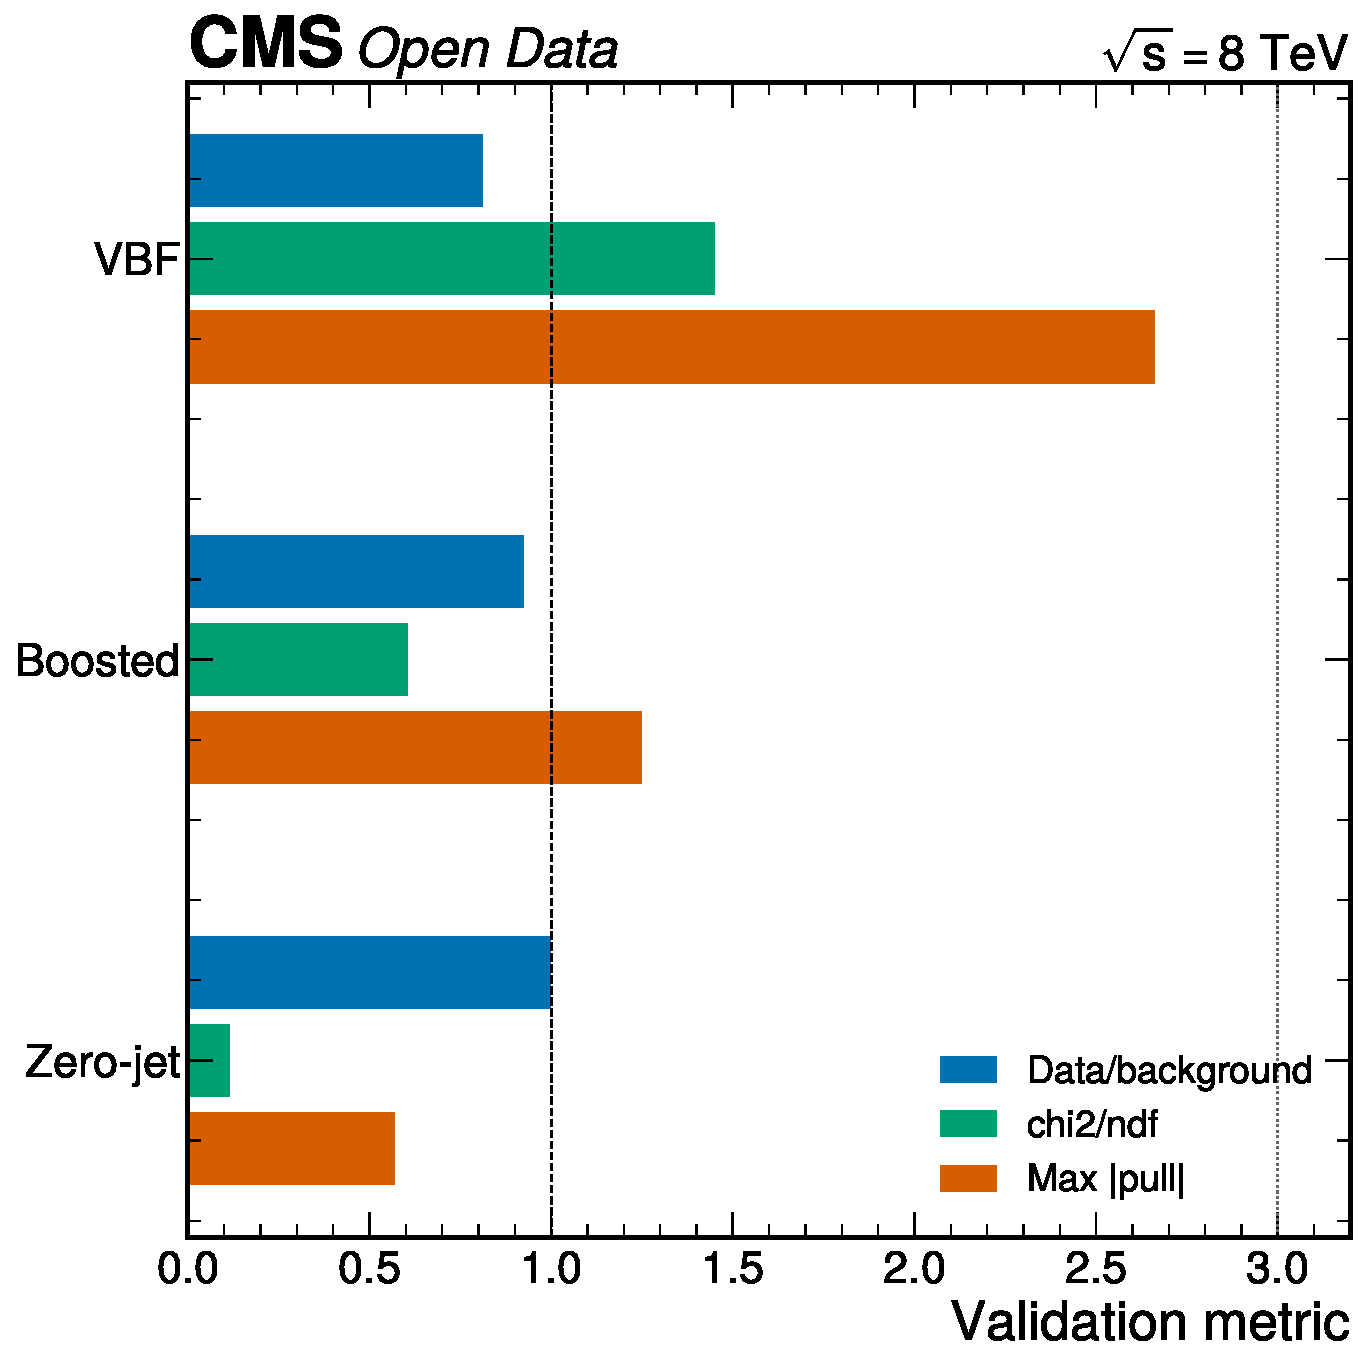
\includegraphics[height=0.35\textheight,width=\linewidth,keepaspectratio,alt={Baseline validation summary. The figure compares data/background, chi2/ndf, and max absolute pull across the final visible-mass categories. It highlights that the combined result passes while VBF carries the largest localized residual tension.}]{figures/phase5_baseline_validation_summary.pdf}}
\caption{Baseline validation summary. The figure compares
data/background, chi2/ndf, and max absolute pull across the final
visible-mass categories. It highlights that the combined result passes
while VBF carries the largest localized residual
tension.}\label{fig:baseline-validation-summary}
\end{figure}

\needspace{4\baselineskip}
\FloatBarrier
\section{Nuisance Parameters and Fit
Health}\label{nuisance-parameters-and-fit-health}

The most important fitted nuisance values are stored in the baseline
result JSON under \texttt{observed\_fit.parameters}. Their values are
reported in prefit sigma units for constrained parameters.

{\def\LTcaptype{none} % do not increment counter
\vspace{1em}
\begin{table}[htbp]
\centering
\small
\begin{tabular}{@{}
lrl@{}}
\toprule\noalign{}
Source & Post-fit value & Status \\
\midrule\noalign{}
Luminosity & -0.107 & Included \\
Tau/open-data acceptance & -0.678 & Included \\
DY/Z normalization & 0.680 & Included \\
W high-mT control & 0.192 & Included \\
VBF background control & -0.580 & Included \\
Same-sign QCD/fake transfer & 0.490 & Included \\
\end{tabular}
\end{table}
}

The DY/Z normalization and tau/open-data acceptance pulls are sizable
but remain within the range where the model can still be interpreted as
a conservative reduced-sample fit. No listed global nuisance exceeds ±1
sigma by a large margin except the known reduced-sample DY/Z pressure.
MC statistical terms are numerous and are listed in the JSON rather than
repeated line-by-line in the main text.

\needspace{0.4\textheight}
\begin{figure}[htbp]
\centering
\pandocbounded{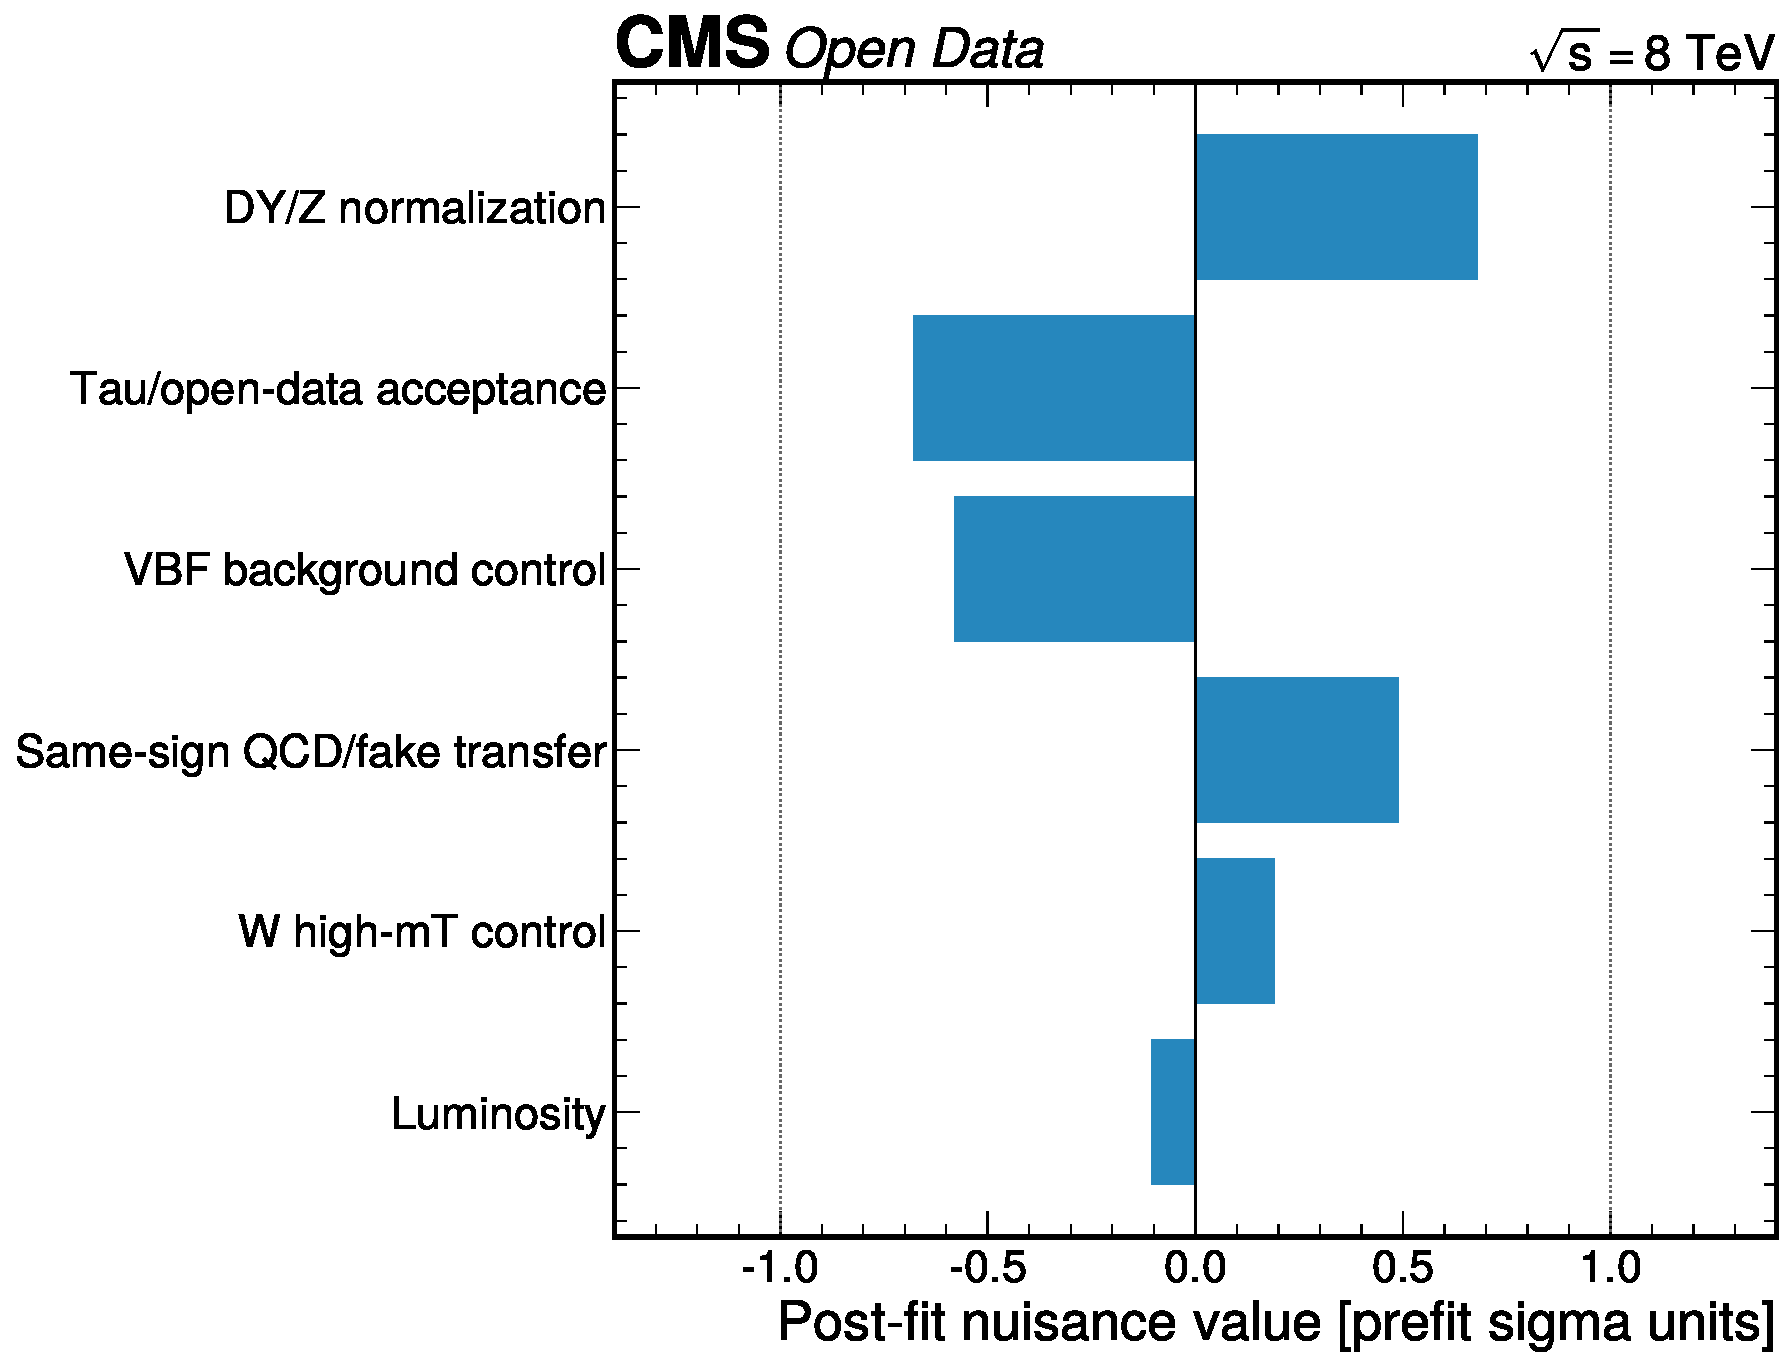
\includegraphics[height=0.35\textheight,width=\linewidth,keepaspectratio,alt={Baseline nuisance pulls. The figure shows the global non-MC-stat nuisance values in the final visible-mass fit. It gives the reader a compact check that the final weak limit is not driven by an obviously pathological pull.}]{figures/phase5_nuisance_pulls_baseline.pdf}}
\caption{Baseline nuisance pulls. The figure shows the global
non-MC-stat nuisance values in the final visible-mass fit. It gives the
reader a compact check that the final weak limit is not driven by an
obviously pathological pull.}\label{fig:nuisance-pulls}
\end{figure}

The expected and validation-stage health checks are retained as context.
The expected Asimov classifier study had median limit 2.904, while the
full-data final baseline has median expected limit 10.7375; this loss of
sensitivity is the cost of using the validated robust model. The 10\%
validation sample had combined score-template data/background 1.232 and
chi2/ndf 1.732, already indicating that aggressive classifier use needed
full-data scrutiny.

\needspace{0.4\textheight}
\begin{figure}[htbp]
\centering
\pandocbounded{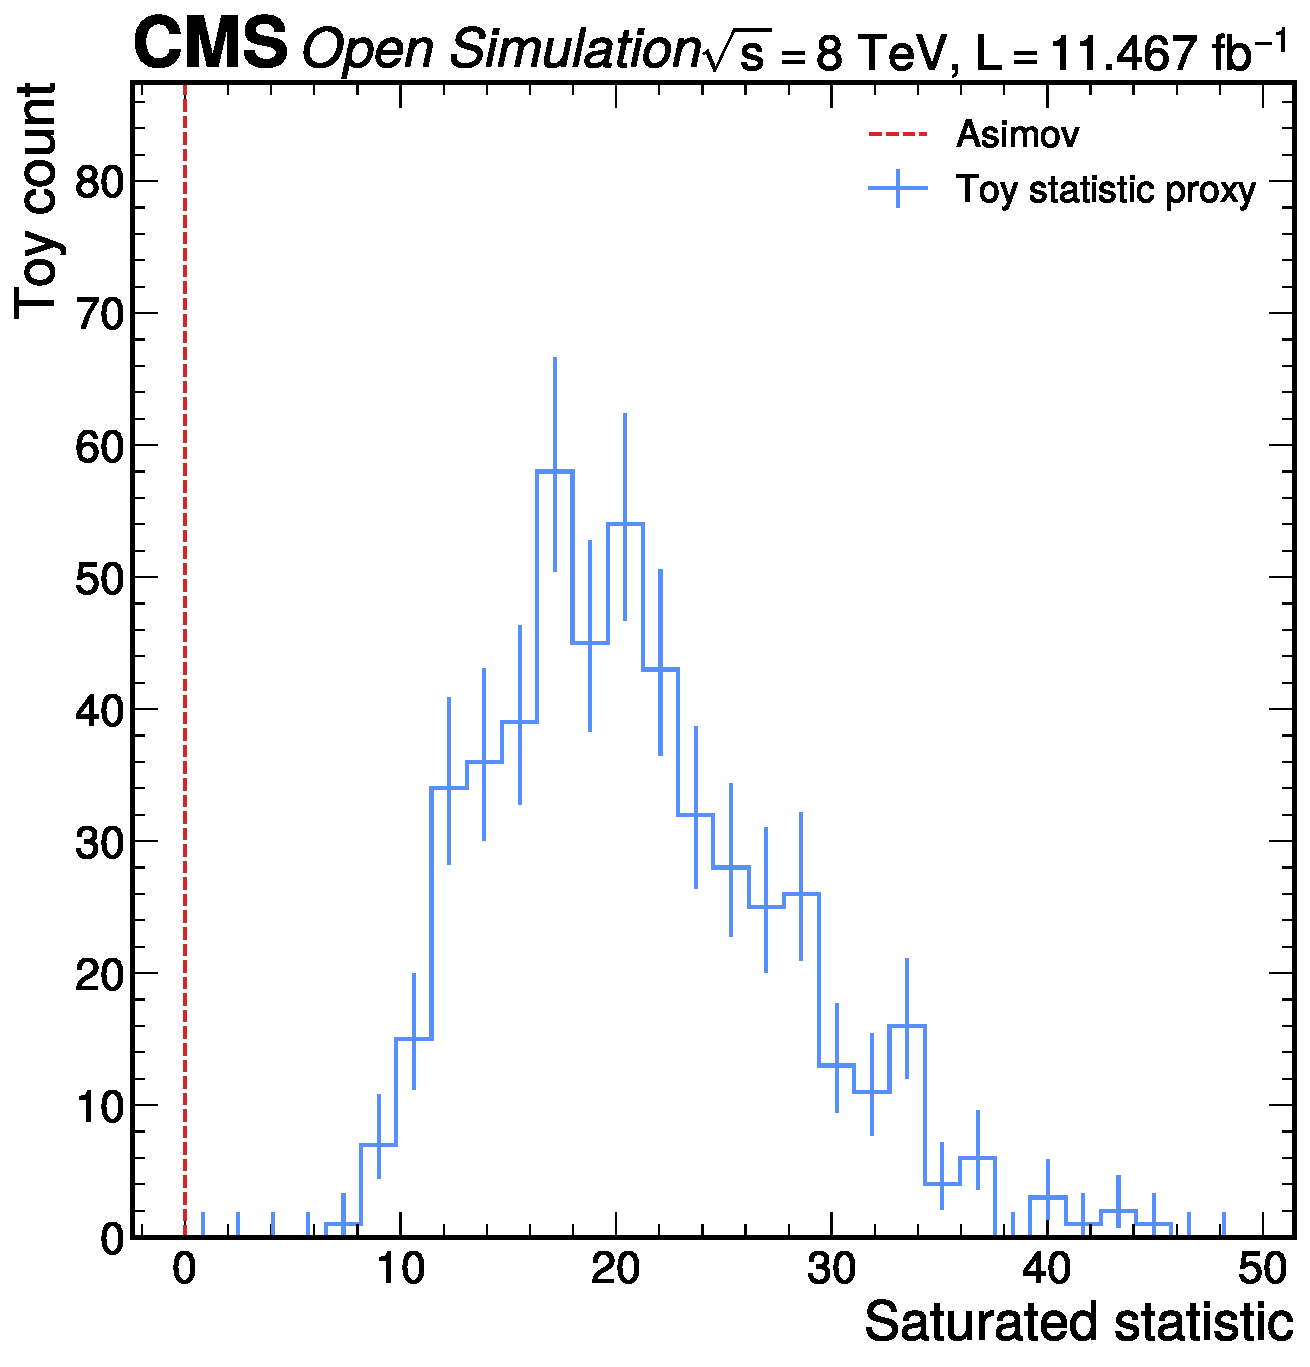
\includegraphics[height=0.35\textheight,width=\linewidth,keepaspectratio,alt={Goodness-of-fit toy study. This expected-stage figure records the available toy-style GoF validation artifact. The final observed baseline note does not claim a full observed-data toy ensemble because no such artifact is available in the current JSON outputs.}]{figures/gof_toys.pdf}}
\caption{Goodness-of-fit toy study. This expected-stage figure records
the available toy-style GoF validation artifact. The final observed
baseline note does not claim a full observed-data toy ensemble because
no such artifact is available in the current JSON
outputs.}\label{fig:gof-toys}
\end{figure}

\needspace{0.4\textheight}
\begin{figure}[htbp]
\centering
\pandocbounded{
\includegraphics[height=0.35\textheight,width=\linewidth,keepaspectratio,alt={Signal-injection recovery. This validation figure documents the available injected-signal recovery study. The final baseline result remains low sensitivity, but the injection artifact shows that the statistical machinery can recover injected signals within the tested setup.}]{figures/signal_injection_recovery.pdf}}
\caption{Signal-injection recovery. This validation figure documents the
available injected-signal recovery study. The final baseline result
remains low sensitivity, but the injection artifact shows that the
statistical machinery can recover injected signals within the tested
setup.}\label{fig:signal-injection}
\end{figure}

\needspace{0.4\textheight}
\begin{figure}[htbp]
\centering
\pandocbounded{
\includegraphics[height=0.35\textheight,width=\linewidth,keepaspectratio,alt={Nuisance audit. This figure summarizes the available nuisance-audit artifact from the inference workflow. It is retained as supporting fit-health context, while the main text reports the final baseline nuisance values from JSON.}]{figures/sensitivity_nuisance_audit.pdf}}
\caption{Nuisance audit. This figure summarizes the available
nuisance-audit artifact from the inference workflow. It is retained as
supporting fit-health context, while the main text reports the final
baseline nuisance values from JSON.}\label{fig:nuisance-audit}
\end{figure}

\needspace{4\baselineskip}
\FloatBarrier
\section{Final Result}\label{final-result}

The final result is the visible-mass baseline only. Its profile fit
gives

\begin{equation}\protect\phantomsection\label{eq:final-muhat}{
\hat{\mu} = 0.4382^{+4.9443}_{-0.4382},
}\end{equation}

with the lower side bounded at zero, and the 95\% CLs upper limit is

\begin{equation}\protect\phantomsection\label{eq:final-limit}{
\mu < 10.7645\quad(95\%~\mathrm{CL}_s),
}\end{equation}

compared with a median expected limit of 10.7375. The discovery
diagnostic is \(Z = 0.0949\) with p-value 0.4622; it is consistent with
the low-sensitivity limit interpretation.

{\def\LTcaptype{none} % do not increment counter
\vspace{1em}
\begin{table}[htbp]
\centering
\small
\begin{tabular}{@{}
lr@{}}
\toprule\noalign{}
Quantity & Final visible-mass result \\
\midrule\noalign{}
Best-fit signal strength & 0.4382 +4.9443 -0.4382 \\
Observed 95\% CLs limit & mu \textless{} 10.7645 \\
Expected 95\% CLs limit, −2 sigma & mu \textless{} 5.4271 \\
Expected 95\% CLs limit, −1 sigma & mu \textless{} 7.4538 \\
Expected 95\% CLs limit, median & mu \textless{} 10.7375 \\
Expected 95\% CLs limit, +1 sigma & mu \textless{} 15.7354 \\
Expected 95\% CLs limit, +2 sigma & mu \textless{} 22.4849 \\
q0 diagnostic Z & 0.0949 \\
Combined data/background & 0.9812 \\
Combined chi2/ndf & 0.7224 \\
\end{tabular}
\end{table}
}

\needspace{0.4\textheight}
\begin{figure}[htbp]
\centering
\pandocbounded{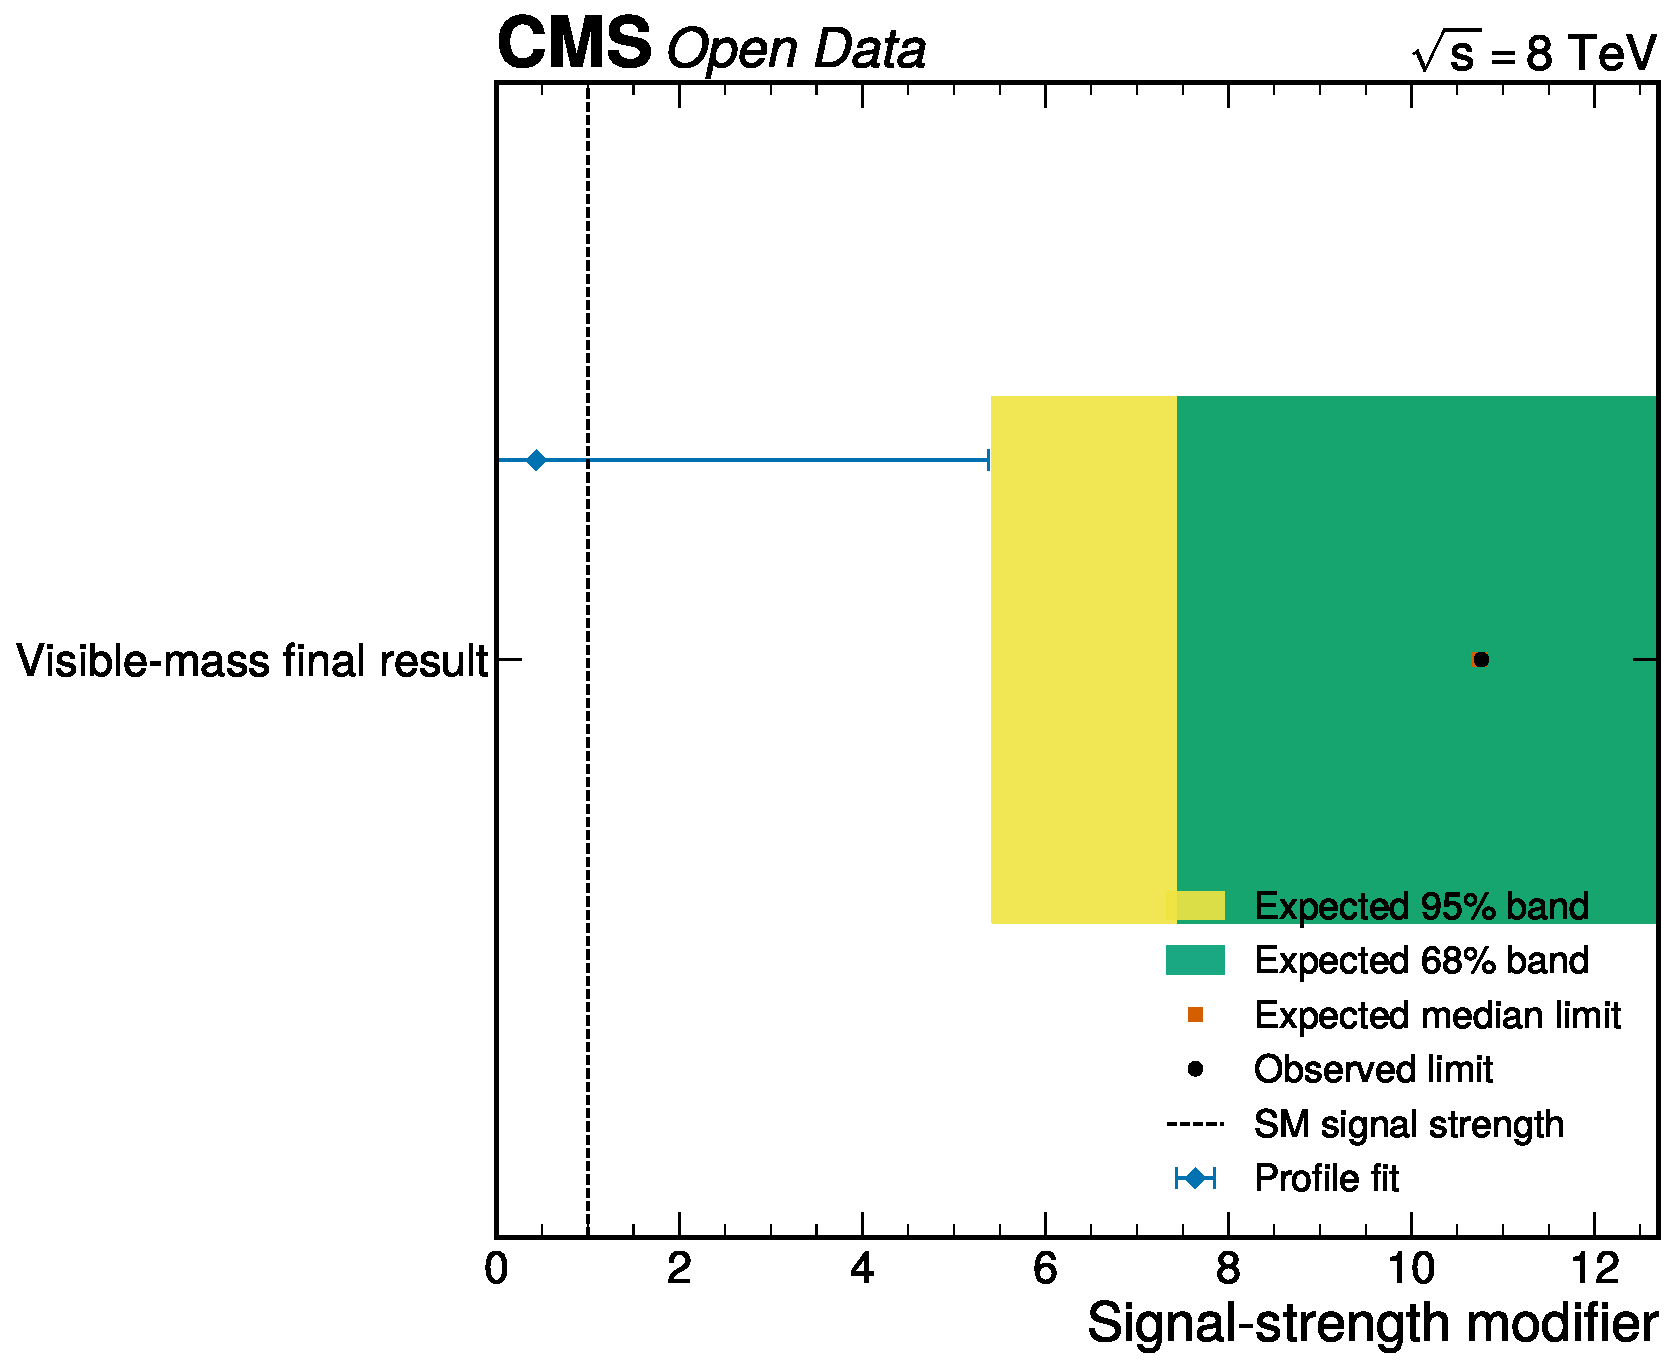
\includegraphics[height=0.35\textheight,width=\linewidth,keepaspectratio,alt={Final baseline limit summary. The figure shows only the validated visible-mass final result with the expected CLs band, observed limit, and profile best-fit interval. No optimized-score value appears in the headline final-result plot.}]{figures/phase5_baseline_limit_summary.pdf}}
\caption{Final baseline limit summary. The figure shows only the
validated visible-mass final result with the expected CLs band, observed
limit, and profile best-fit interval. No optimized-score value appears
in the headline final-result plot.}\label{fig:baseline-limit}
\end{figure}

\needspace{4\baselineskip}
\FloatBarrier
\section{Rejected Classifier Diagnostic}\label{sec:rejected-classifier}

The optimized calibrated-score model is not a final result. It is
retained here because it explains why the analysis does not use the best
expected-only sensitivity model. The model has median expected limit
1.9735, but on full observed data it gives
\texttt{mu\ =\ 38.3802\ +7.0346\ -6.1157}, observed limit
\texttt{mu\ \textless{}\ 50.0000}, and q0 diagnostic
\texttt{Z\ =\ 12.4698}.

{\def\LTcaptype{none} % do not increment counter
\vspace{1em}
\begin{table}[htbp]
\centering
\small
\begin{tabular}{@{}
>{\raggedright\arraybackslash}p{(\linewidth - 4\tabcolsep) * \real{0.3000}}
  >{\raggedleft\arraybackslash}p{(\linewidth - 4\tabcolsep) * \real{0.4000}}
  >{\raggedright\arraybackslash}p{(\linewidth - 4\tabcolsep) * \real{0.3000}}@{}}
\toprule\noalign{}
\begin{minipage}[b]{\linewidth}\raggedright
Diagnostic
\end{minipage} & \begin{minipage}[b]{\linewidth}\raggedleft
Value
\end{minipage} & \begin{minipage}[b]{\linewidth}\raggedright
Interpretation
\end{minipage} \\
\midrule\noalign{}
Expected median 95\% CLs limit & mu \textless{} 1.9735 & Would be
sensitive if observed modelling passed \\
Observed 95\% CLs limit & mu \textless{} 50.0000 & Hits scan boundary;
diagnostic failure \\
Best-fit signal strength & 38.3802 +7.0346 -6.1157 & Far outside
reduced-analysis plausibility \\
q0 diagnostic & Z = 12.4698 & Rejected, not a discovery claim \\
Combined data/background & 0.6631 & Gross normalization mismatch \\
Combined chi2/ndf & 2.4808 & Shape/normalization validation
diagnostic \\
Validation gate & fail & The optimized classifier is rejected if it has
a boundary-like limit, a large q0 diagnostic, or a gross combined
normalization mismatch. \\
\end{tabular}
\end{table}
}

The category fits also indicate model breakdown rather than
category-level consistency. The zero-jet category reaches the scan
boundary, and VBF/boosted fitted values are several times the Standard
Model strength. These values are not used in the abstract, final-result
table, conclusion, or published-context comparison.

\needspace{0.4\textheight}
\begin{figure}[htbp]
\centering
\pandocbounded{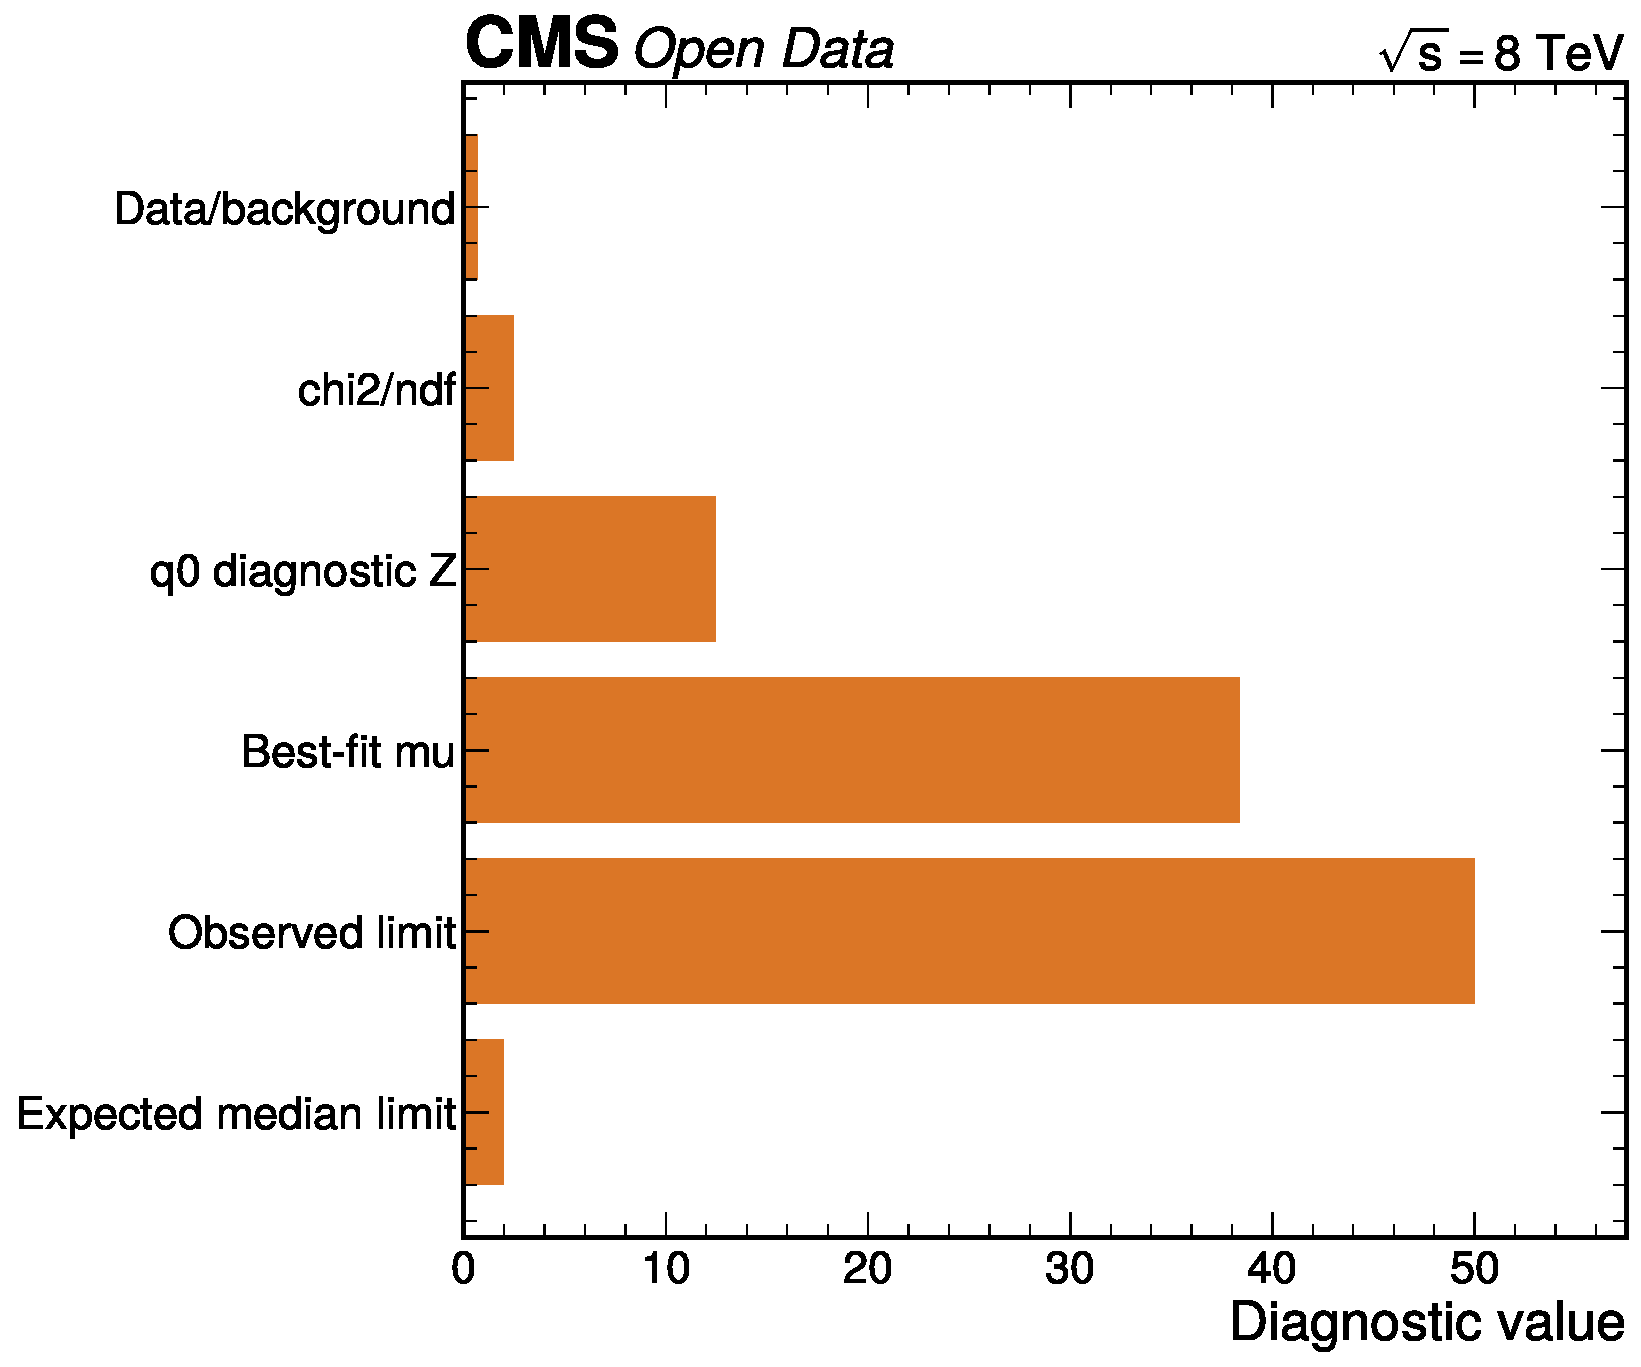
\includegraphics[height=0.35\textheight,width=\linewidth,keepaspectratio,alt={Rejected classifier diagnostic summary. The figure collects the failed optimized-score validation metrics in one diagnostic plot. It is intentionally separated from the final-result section so the failed model is not mistaken for this analysis's physics result.}]{figures/phase5_rejected_score_diagnostics.pdf}}
\caption{Rejected classifier diagnostic summary. The figure collects the
failed optimized-score validation metrics in one diagnostic plot. It is
intentionally separated from the final-result section so the failed
model is not mistaken for this analysis's physics
result.}\label{fig:rejected-score-diagnostics}
\end{figure}

\needspace{0.4\textheight}
\begin{figure}[htbp]
\centering
\pandocbounded{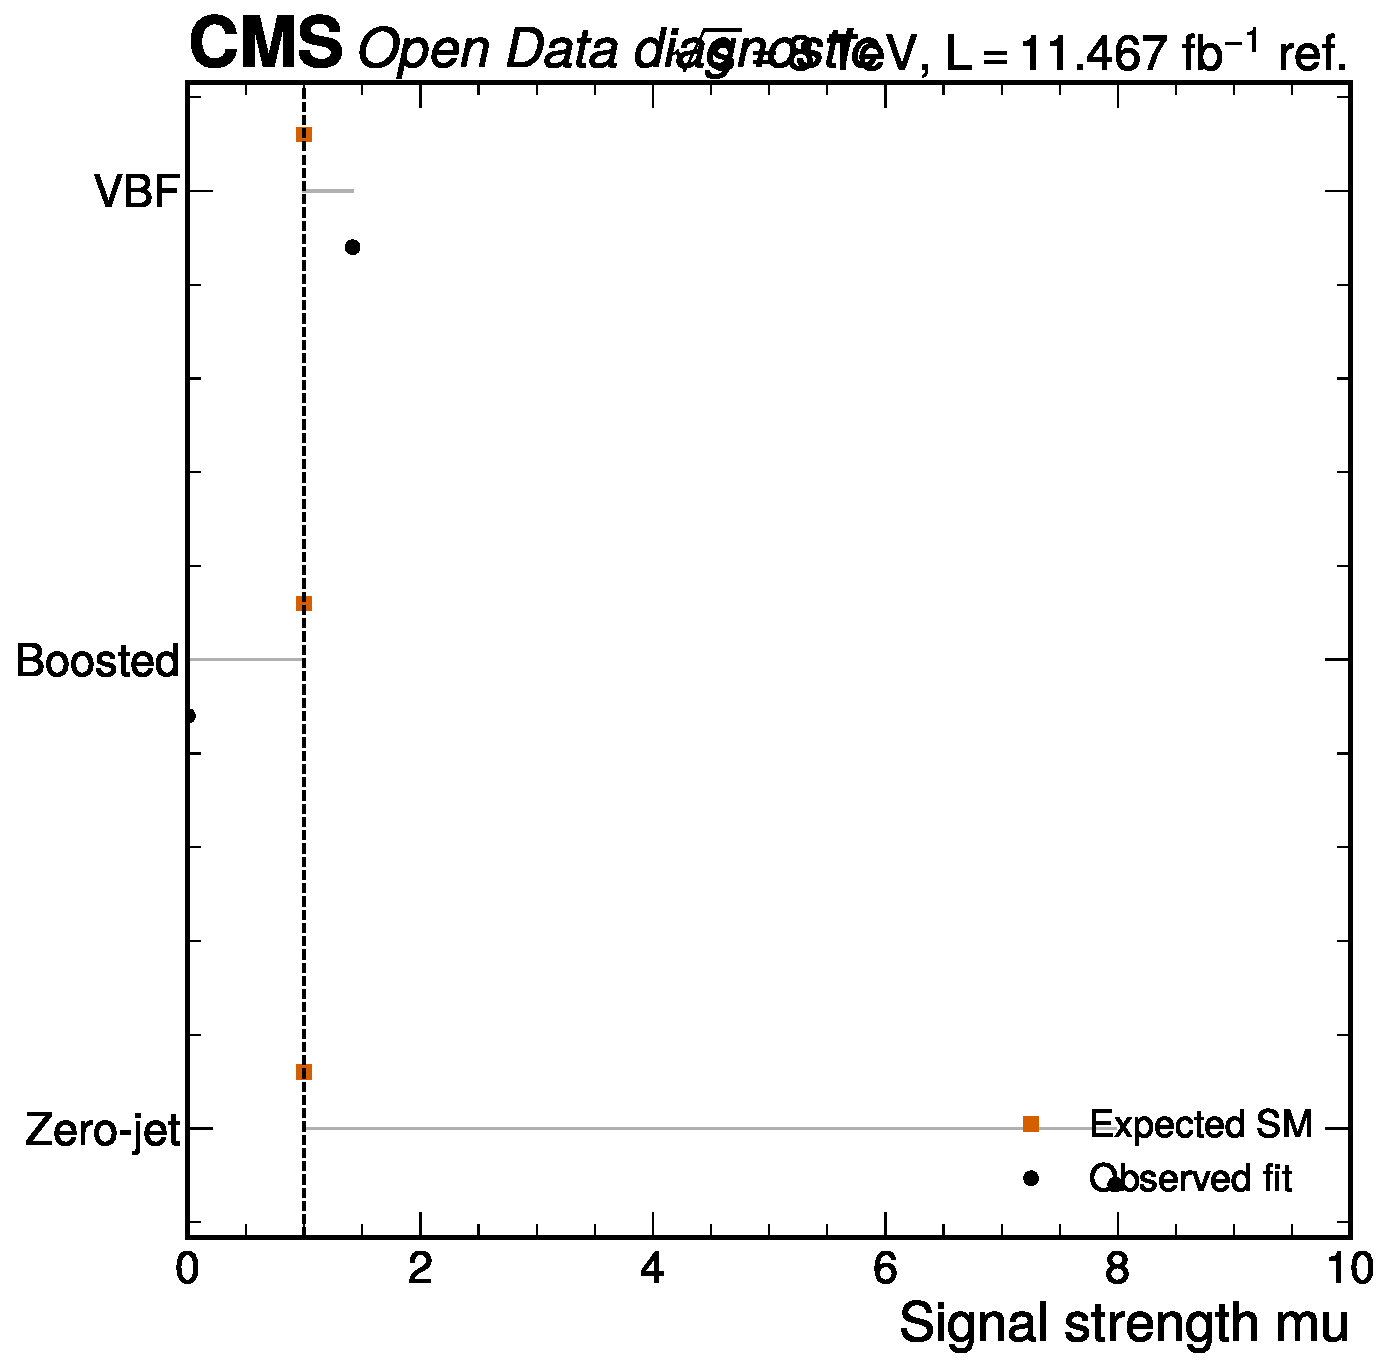
\includegraphics[height=0.35\textheight,width=\linewidth,keepaspectratio,alt={Rejected classifier category fits. The figure shows the single-category signal-strength diagnostics for the optimized classifier model. The large fitted values, including boundary behavior, are evidence for rejection of the classifier result rather than evidence for Higgs production.}]{figures/phase5_category_mu_comparison.pdf}}
\caption{Rejected classifier category fits. The figure shows the
single-category signal-strength diagnostics for the optimized classifier
model. The large fitted values, including boundary behavior, are
evidence for rejection of the classifier result rather than evidence for
Higgs production.}\label{fig:rejected-category-mu}
\end{figure}

\needspace{4\baselineskip}
\FloatBarrier
\section{Comparison With Published
Context}\label{comparison-with-published-context}

Published CMS and ATLAS+CMS H to tau tau analyses use more channels,
fuller calibrations, embedded backgrounds, and substantially richer
systematic programs than this reduced Open Data study (CMS Collaboration
2014, 2018; ATLAS and CMS Collaborations 2016). The comparison is
therefore interpretive, not a validation target. The final result is
compatible with published signal strengths only in the weak sense that
its uncertainty and upper limit are too large to distinguish \(\mu=1\)
from background.

The pull of the final best fit relative to the CMS Run 1
\(\mu = 0.78 \pm 0.27\) value is not meaningful as a precision
comparison because this analysis has an asymmetric interval with a lower
physical boundary. Using the upward uncertainty as a conservative scale
gives \((0.438-0.78)/4.944 = -0.07\) standard deviations. Relative to
the ATLAS+CMS global \(\mu = 1.09 \pm 0.11\), the same conservative
comparison gives \((0.438-1.09)/4.944 = -0.13\) standard deviations.
These small pulls reflect low resolving power, not precision agreement.

{\def\LTcaptype{none} % do not increment counter
\vspace{1em}
\begin{table}[htbp]
\centering
\small
\begin{tabular}{@{}
>{\raggedright\arraybackslash}p{(\linewidth - 6\tabcolsep) * \real{0.2500}}
  >{\raggedright\arraybackslash}p{(\linewidth - 6\tabcolsep) * \real{0.2500}}
  >{\raggedright\arraybackslash}p{(\linewidth - 6\tabcolsep) * \real{0.2500}}
  >{\raggedright\arraybackslash}p{(\linewidth - 6\tabcolsep) * \real{0.2500}}@{}}
\toprule\noalign{}
\begin{minipage}[b]{\linewidth}\raggedright
Result
\end{minipage} & \begin{minipage}[b]{\linewidth}\raggedright
Scope
\end{minipage} & \begin{minipage}[b]{\linewidth}\raggedright
Signal-strength or limit
\end{minipage} & \begin{minipage}[b]{\linewidth}\raggedright
Interpretation
\end{minipage} \\
\midrule\noalign{}
This analysis & 8 TeV reduced mu tau\_h visible-mass fit & mu = 0.4382
+4.9443 -0.4382; 95\% CLs mu \textless{} 10.7645; median expected 95\%
CLs mu \textless{} 10.7375 & Low-sensitivity Open Data upper limit \\
CMS Run 1 & 7+8 TeV multi-channel & mu = 0.78 ± 0.27; observed 3.2 sigma
& Evidence-level publication analysis \\
CMS 2018 & 13 TeV multi-channel & mu about 1.09; observed 4.9 sigma &
Observation in 2016 data \\
CMS combined in 2018 paper & CMS 7+8+13 TeV & observed 5.9 sigma & CMS
observation context \\
ATLAS+CMS Run 1 & 7+8 TeV global Higgs combination & global mu = 1.09 ±
0.11 & Precision Higgs-rate context \\
PDG/HXSWG SM & Standard Model normalization & BR(H to tau tau) about
6.3\% & Defines the \texttt{mu\ =\ 1} convention \\
\end{tabular}
\end{table}
}

The validated result cannot exclude or discover a Standard
Model-strength Higgs signal in this reduced setup. Its expected limit
near 10.74 says that even a perfect background-like observation would
only constrain signals roughly an order of magnitude above the SM rate.

\needspace{4\baselineskip}
\FloatBarrier
\section{Limitations}\label{limitations}

The most important limitation is missing reduced-sample content. No
embedded \(Z\to\tau\tau\), diboson, single-top, QCD multijet MC,
W4/inclusive W+jets, associated-Higgs, or H to WW reduced files are
available in the localized mirror used here. These absences limit both
sensitivity and systematic realism.

The second limitation is the lack of source-by-source baseline impact
refits in the current machine-readable outputs. The final note reports
implemented nuisance values, fitted nuisance pulls, and validation
metrics, but it does not invent per-source impacts. A future Phase 4
extension should produce an impact JSON by fixing or shifting each
nuisance in the final baseline workspace and recording the change in
\texttt{mu} and the CLs limit.

The third limitation is validation coverage. The final baseline passes
the available combined and category checks, but no full observed-data
GoF toy ensemble is stored. The VBF category has a residual local
tension and the zero-jet chi2/ndf is low. Both effects should be
revisited with fuller control-region coverage before making stronger
physics claims.

\needspace{4\baselineskip}
\FloatBarrier
\section{Reproduction Contract}\label{reproduction-contract}

The final documents are generated from the current JSON artifacts and
pyhf workspaces. A reader with the repository can rebuild the package
through pixi:

{\def\LTcaptype{none} % do not increment counter
\vspace{1em}
\begin{table}[htbp]
\centering
\small
\begin{tabular}{@{}
>{\raggedright\arraybackslash}p{(\linewidth - 2\tabcolsep) * \real{0.5000}}
  >{\raggedright\arraybackslash}p{(\linewidth - 2\tabcolsep) * \real{0.5000}}@{}}
\toprule\noalign{}
\begin{minipage}[b]{\linewidth}\raggedright
Command
\end{minipage} & \begin{minipage}[b]{\linewidth}\raggedright
Purpose
\end{minipage} \\
\midrule\noalign{}
\texttt{pixi\ run\ phase2-explore} & Reproduce sample inventory and
exploration artifacts \\
\texttt{pixi\ run\ phase3-all} & Rebuild selected events, selection
figures, and sensitivity artifacts \\
\texttt{pixi\ run\ phase4a-all} & Rebuild expected-only workspaces and
validation \\
\texttt{pixi\ run\ phase4b-all} & Rebuild 10\% validation artifacts \\
\texttt{pixi\ run\ phase4c-all} & Rebuild full-data observed
artifacts \\
\texttt{pixi\ run\ phase5-docs} & Regenerate this note, PRL draft,
references, and Phase 5 figures \\
\texttt{pixi\ run\ lint-plots} & Run deterministic plot-standard
linting \\
\texttt{pixi\ run\ build-pdf} & Rebuild the final analysis note PDF from
markdown \\
\end{tabular}
\end{table}
}

The machine-readable numerical sources for the final result are:

{\def\LTcaptype{none} % do not increment counter
\vspace{1em}
\begin{table}[htbp]
\centering
\small
\begin{tabular}{@{}
ll@{}}
\toprule\noalign{}
Quantity & Artifact \\
\midrule\noalign{}
Final fit and validation & baseline result JSON \\
Final workspace & \texttt{pyhf\_workspace\_baseline\_visible.json} \\
Visible-mass yields & \texttt{baseline\_visible\_yields.json} \\
Final role metadata & \texttt{observed\_results.json} \\
W high-mT scale & \texttt{wjets\_highmt\_scale\_full.json} \\
VBF background scale & \texttt{vbf\_background\_scale.json} \\
QCD/fake estimates & \texttt{qcd\_sideband\_estimates.json} \\
Category diagnostics & \texttt{category\_mu\_comparison.json} \\
\end{tabular}
\end{table}
}

\needspace{4\baselineskip}
\FloatBarrier
\section{Appendix A: Bin-Level Baseline
Yields}\label{appendix-a-bin-level-baseline-yields}

The tables below expose the bin-level values used in the regenerated
visible-mass validation plots. They are copied from
\texttt{baseline\_visible\_yields.json} and allow the reader to
reproduce the ratios in Figure~\ref{fig:baseline-visible-vbf},
Figure~\ref{fig:baseline-visible-boosted}, and
Figure~\ref{fig:baseline-visible-zero}.

\needspace{4\baselineskip}
\subsection{VBF Bin Yields}\label{vbf-bin-yields}

{\def\LTcaptype{none} % do not increment counter
\vspace{1em}
\begin{table}[htbp]
\centering
\small
\begin{tabular}{@{}
>{\raggedright\arraybackslash}p{(\linewidth - 10\tabcolsep) * \real{0.1304}}
  >{\raggedleft\arraybackslash}p{(\linewidth - 10\tabcolsep) * \real{0.1739}}
  >{\raggedleft\arraybackslash}p{(\linewidth - 10\tabcolsep) * \real{0.1739}}
  >{\raggedleft\arraybackslash}p{(\linewidth - 10\tabcolsep) * \real{0.1739}}
  >{\raggedleft\arraybackslash}p{(\linewidth - 10\tabcolsep) * \real{0.1739}}
  >{\raggedleft\arraybackslash}p{(\linewidth - 10\tabcolsep) * \real{0.1739}}@{}}
\toprule\noalign{}
\begin{minipage}[b]{\linewidth}\raggedright
Visible mass bin {[}GeV{]}
\end{minipage} & \begin{minipage}[b]{\linewidth}\raggedleft
Data
\end{minipage} & \begin{minipage}[b]{\linewidth}\raggedleft
Background
\end{minipage} & \begin{minipage}[b]{\linewidth}\raggedleft
QCD/fake
\end{minipage} & \begin{minipage}[b]{\linewidth}\raggedleft
Signal
\end{minipage} & \begin{minipage}[b]{\linewidth}\raggedleft
Data/background
\end{minipage} \\
\midrule\noalign{}
0-60 & 32 & 39.59 & 5.828 & 0.420 & 0.808 \\
60-80 & 23 & 19.42 & 5.032 & 0.808 & 1.184 \\
80-100 & 4 & 14.04 & 3.154 & 0.297 & 0.285 \\
100-120 & 5 & 5.84 & 0.000 & 0.063 & 0.856 \\
120-160 & 6 & 8.24 & 0.000 & 0.002 & 0.728 \\
160-250 & 8 & 9.14 & 3.733 & 0.000 & 0.875 \\
\end{tabular}
\end{table}
}

\needspace{4\baselineskip}
\subsection{Boosted Bin Yields}\label{boosted-bin-yields}

{\def\LTcaptype{none} % do not increment counter
\vspace{1em}
\begin{table}[htbp]
\centering
\small
\begin{tabular}{@{}
>{\raggedright\arraybackslash}p{(\linewidth - 10\tabcolsep) * \real{0.1304}}
  >{\raggedleft\arraybackslash}p{(\linewidth - 10\tabcolsep) * \real{0.1739}}
  >{\raggedleft\arraybackslash}p{(\linewidth - 10\tabcolsep) * \real{0.1739}}
  >{\raggedleft\arraybackslash}p{(\linewidth - 10\tabcolsep) * \real{0.1739}}
  >{\raggedleft\arraybackslash}p{(\linewidth - 10\tabcolsep) * \real{0.1739}}
  >{\raggedleft\arraybackslash}p{(\linewidth - 10\tabcolsep) * \real{0.1739}}@{}}
\toprule\noalign{}
\begin{minipage}[b]{\linewidth}\raggedright
Visible mass bin {[}GeV{]}
\end{minipage} & \begin{minipage}[b]{\linewidth}\raggedleft
Data
\end{minipage} & \begin{minipage}[b]{\linewidth}\raggedleft
Background
\end{minipage} & \begin{minipage}[b]{\linewidth}\raggedleft
QCD/fake
\end{minipage} & \begin{minipage}[b]{\linewidth}\raggedleft
Signal
\end{minipage} & \begin{minipage}[b]{\linewidth}\raggedleft
Data/background
\end{minipage} \\
\midrule\noalign{}
0-60 & 971 & 974.62 & 135.863 & 1.818 & 0.996 \\
60-80 & 561 & 687.29 & 67.623 & 3.898 & 0.816 \\
80-100 & 243 & 256.01 & 35.400 & 2.596 & 0.949 \\
100-120 & 155 & 146.36 & 28.825 & 0.785 & 1.059 \\
120-160 & 149 & 172.98 & 29.470 & 0.039 & 0.861 \\
160-250 & 104 & 127.14 & 28.396 & 0.035 & 0.818 \\
\end{tabular}
\end{table}
}

\needspace{4\baselineskip}
\subsection{Zero-Jet Bin Yields}\label{zero-jet-bin-yields}

{\def\LTcaptype{none} % do not increment counter
\vspace{1em}
\begin{table}[htbp]
\centering
\small
\begin{tabular}{@{}
>{\raggedright\arraybackslash}p{(\linewidth - 10\tabcolsep) * \real{0.1304}}
  >{\raggedleft\arraybackslash}p{(\linewidth - 10\tabcolsep) * \real{0.1739}}
  >{\raggedleft\arraybackslash}p{(\linewidth - 10\tabcolsep) * \real{0.1739}}
  >{\raggedleft\arraybackslash}p{(\linewidth - 10\tabcolsep) * \real{0.1739}}
  >{\raggedleft\arraybackslash}p{(\linewidth - 10\tabcolsep) * \real{0.1739}}
  >{\raggedleft\arraybackslash}p{(\linewidth - 10\tabcolsep) * \real{0.1739}}@{}}
\toprule\noalign{}
\begin{minipage}[b]{\linewidth}\raggedright
Visible mass bin {[}GeV{]}
\end{minipage} & \begin{minipage}[b]{\linewidth}\raggedleft
Data
\end{minipage} & \begin{minipage}[b]{\linewidth}\raggedleft
Background
\end{minipage} & \begin{minipage}[b]{\linewidth}\raggedleft
QCD/fake
\end{minipage} & \begin{minipage}[b]{\linewidth}\raggedleft
Signal
\end{minipage} & \begin{minipage}[b]{\linewidth}\raggedleft
Data/background
\end{minipage} \\
\midrule\noalign{}
0-60 & 3559 & 3549.55 & 731.797 & 2.560 & 1.003 \\
60-80 & 3475 & 3527.74 & 408.490 & 6.047 & 0.985 \\
80-100 & 772 & 729.65 & 179.425 & 4.651 & 1.058 \\
100-120 & 276 & 279.06 & 97.238 & 1.073 & 0.989 \\
120-160 & 245 & 259.12 & 113.731 & 0.005 & 0.945 \\
160-250 & 124 & 111.69 & 38.964 & 0.005 & 1.110 \\
\end{tabular}
\end{table}
}

\needspace{4\baselineskip}
\FloatBarrier
\section{Appendix B: Validation Bin Ratios and
Pulls}\label{appendix-b-validation-bin-ratios-and-pulls}

{\def\LTcaptype{none} % do not increment counter
\vspace{1em}
\begin{table}[htbp]
\centering
\small
\begin{tabular}{@{}
>{\raggedright\arraybackslash}p{(\linewidth - 4\tabcolsep) * \real{0.3333}}
  >{\raggedright\arraybackslash}p{(\linewidth - 4\tabcolsep) * \real{0.3333}}
  >{\raggedright\arraybackslash}p{(\linewidth - 4\tabcolsep) * \real{0.3333}}@{}}
\toprule\noalign{}
\begin{minipage}[b]{\linewidth}\raggedright
Category
\end{minipage} & \begin{minipage}[b]{\linewidth}\raggedright
Bin ratios
\end{minipage} & \begin{minipage}[b]{\linewidth}\raggedright
Pulls
\end{minipage} \\
\midrule\noalign{}
VBF & 0.808, 1.184, 0.285, 0.856, 0.728, 0.875 & -0.78, 0.56, -2.66,
-0.31, -0.72, -0.29 \\
Boosted & 0.996, 0.816, 0.949, 1.059, 0.861, 0.818 & -0.03, -1.25,
-0.32, 0.34, -0.84, -1.07 \\
Zero-jet & 1.003, 0.985, 1.058, 0.989, 0.945, 1.110 & 0.02, -0.11, 0.44,
-0.07, -0.38, 0.57 \\
\end{tabular}
\end{table}
}

\needspace{4\baselineskip}
\FloatBarrier
\section{Appendix C: Numeric Consistency
Statement}\label{appendix-c-numeric-consistency-statement}

The final AN and PRL quote baseline numbers from JSON fields only. The
best-fit value and profile interval come from
\texttt{observed\_fit.profile\_mu\_interval} in the baseline result
JSON; the CLs limits come from
\texttt{observed\_fit.observed\_upper\_limit}; validation metrics come
from \texttt{validation\_summary}; and visible-mass bin yields come from
\texttt{baseline\_visible\_yields.json}. The optimized classifier values
appear only in Section~\ref{sec:rejected-classifier} and the corresponding
diagnostic JSON/figure.

\needspace{4\baselineskip}
\FloatBarrier
\section{Appendix D: Supporting Validation
Figures}\label{appendix-d-supporting-validation-figures}

This appendix collects additional artifact-backed figures that support
the final model choice and reproduce the analysis chain from input
objects to the retained visible-mass fit. These figures are not used to
quote additional physics results; they document why the final result is
intentionally limited to a weak visible-mass CLs limit and why more
aggressive observables are not promoted to the headline result.

\needspace{0.4\textheight}
\begin{figure}[htbp]
\centering
\pandocbounded{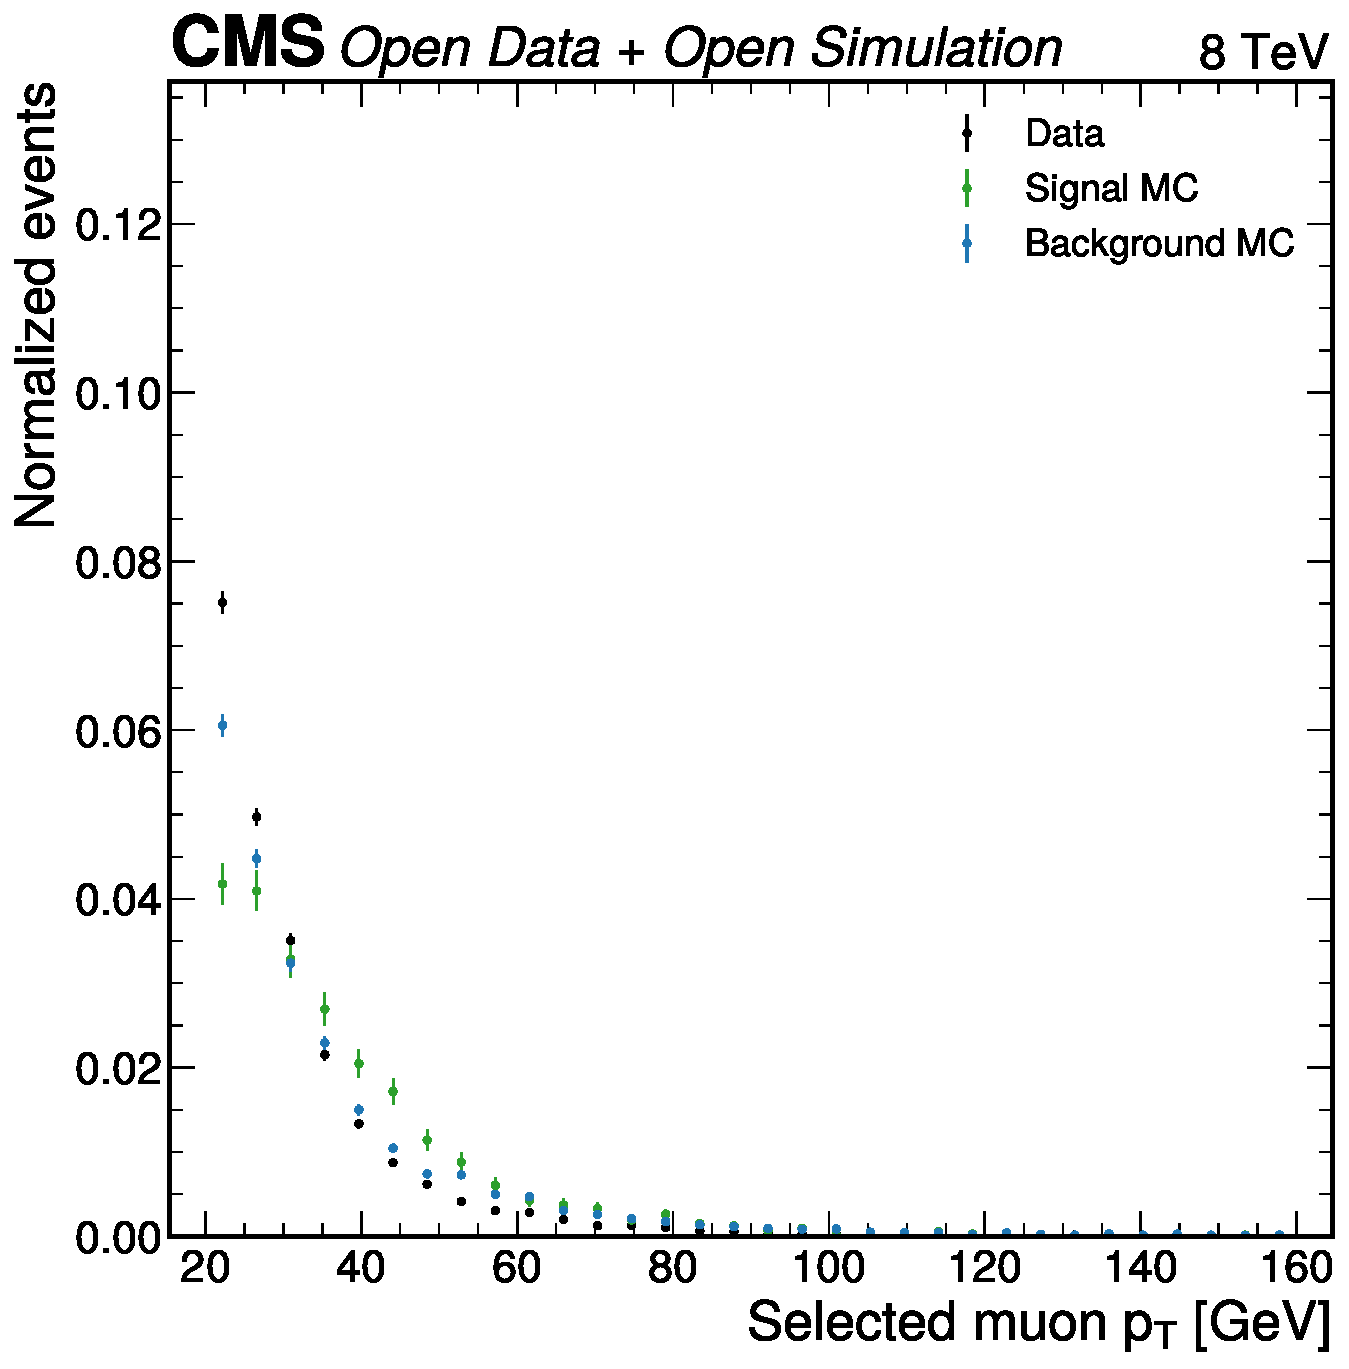
\includegraphics[height=0.35\textheight,width=\linewidth,keepaspectratio,alt={Muon transverse-momentum preselection comparison. This figure checks the reconstructed muon leg in the selected reduced samples. The agreement is not used as a standalone calibration, but it supports the use of the common muon selection in all final categories.}]{figures/mu_pt.pdf}}
\caption{Muon transverse-momentum preselection comparison. This figure
checks the reconstructed muon leg in the selected reduced samples. The
agreement is not used as a standalone calibration, but it supports the
use of the common muon selection in all final
categories.}\label{fig:app-mu-pt}
\end{figure}

\needspace{0.4\textheight}
\begin{figure}[htbp]
\centering
\pandocbounded{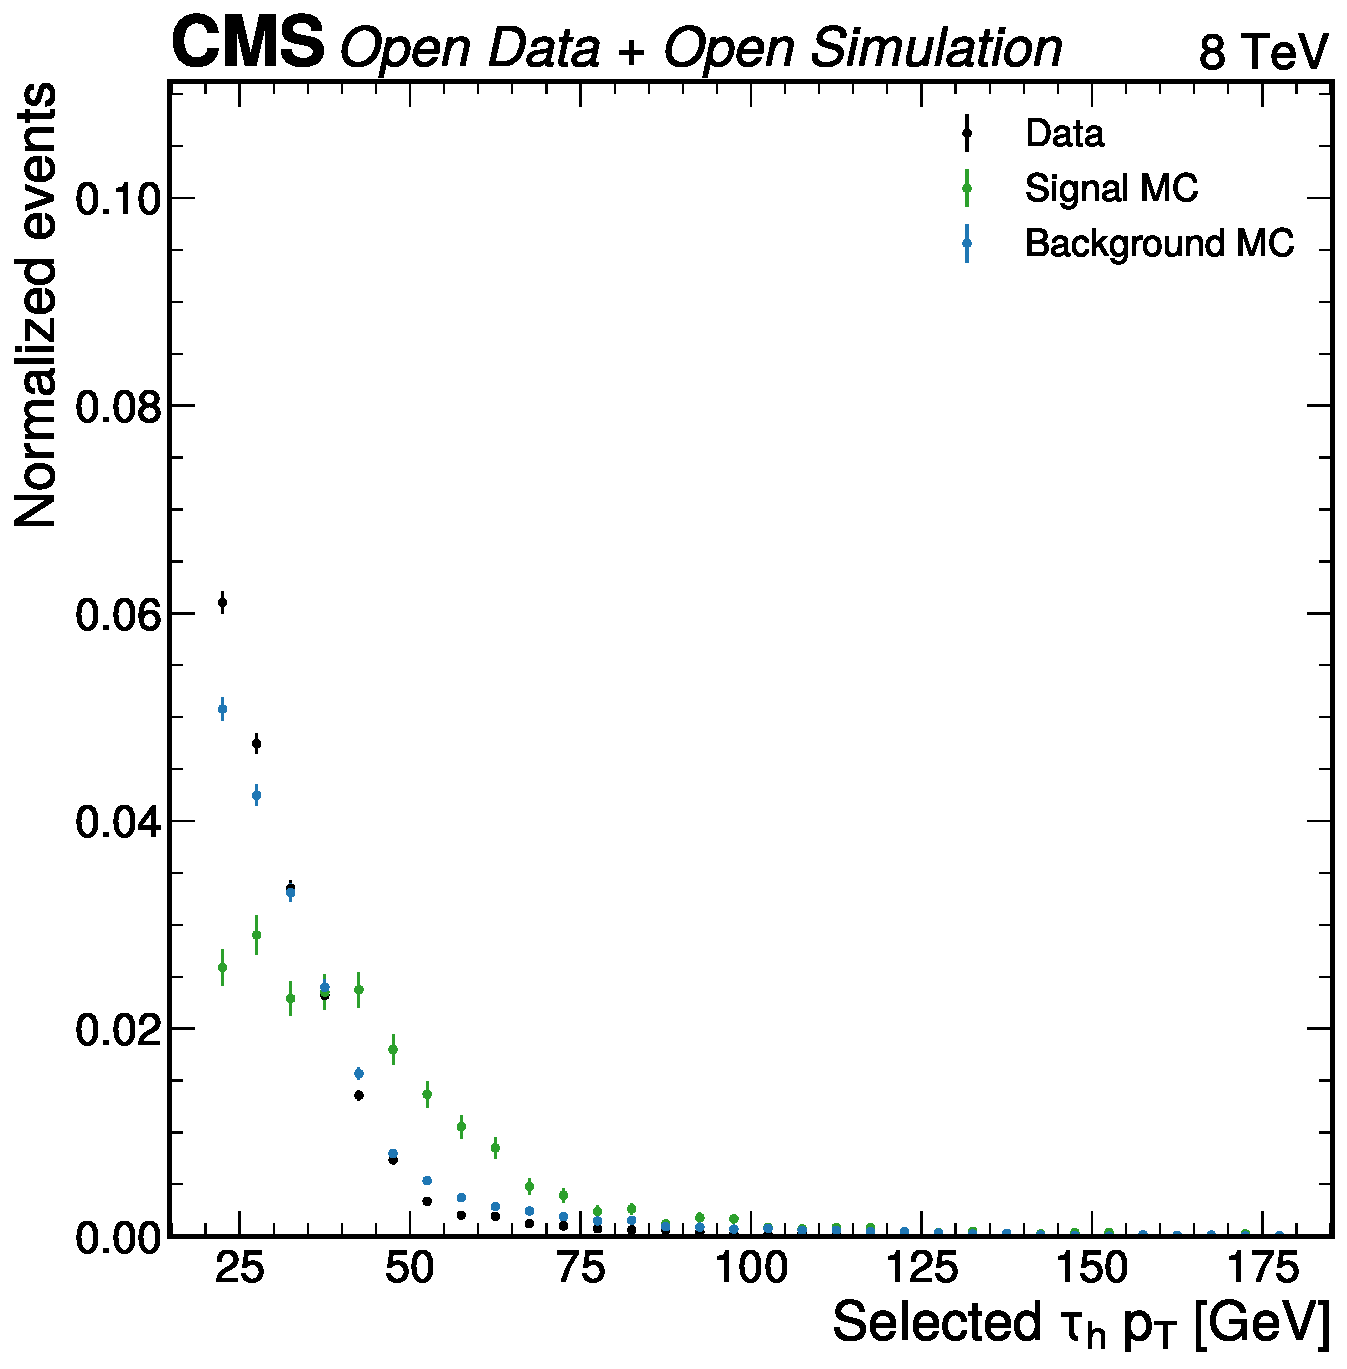
\includegraphics[height=0.35\textheight,width=\linewidth,keepaspectratio,alt={Hadronic-tau transverse-momentum preselection comparison. This figure checks the tau\_h leg after the loose public-object acceptance and tight anti-muon requirement. The final analysis assigns a tau/open-data acceptance nuisance because the public reduced sample does not include the full trigger and tau scale-factor program.}]{figures/tau_pt.pdf}}
\caption{Hadronic-tau transverse-momentum preselection comparison. This
figure checks the tau\_h leg after the loose public-object acceptance
and tight anti-muon requirement. The final analysis assigns a
tau/open-data acceptance nuisance because the public reduced sample does
not include the full trigger and tau scale-factor
program.}\label{fig:app-tau-pt}
\end{figure}

\needspace{0.4\textheight}
\begin{figure}[htbp]
\centering
\pandocbounded{
\includegraphics[height=0.35\textheight,width=\linewidth,keepaspectratio,alt={Missing transverse momentum comparison. This figure checks the missing-momentum observable before it enters the transverse-mass and add-MET cross-check definitions. It motivates treating add-MET based observables as diagnostics rather than replacing the validated visible-mass result.}]{figures/met_pt.pdf}}
\caption{Missing transverse momentum comparison. This figure checks the
missing-momentum observable before it enters the transverse-mass and
add-MET cross-check definitions. It motivates treating add-MET based
observables as diagnostics rather than replacing the validated
visible-mass result.}\label{fig:app-met-pt}
\end{figure}

\needspace{0.4\textheight}
\begin{figure}[htbp]
\centering
\pandocbounded{
\includegraphics[height=0.35\textheight,width=\linewidth,keepaspectratio,alt={Muon-MET transverse-mass comparison. This distribution defines the signal and W-control regions used by the final workflow. The separation between the low-mT signal region and high-mT control region underlies the W+jets normalization factor in eq.~.}]{figures/mt_mu_met.pdf}}
\caption{Muon-MET transverse-mass comparison. This distribution defines
the signal and W-control regions used by the final workflow. The
separation between the low-mT signal region and high-mT control region
underlies the W+jets normalization factor in
Equation~\ref{eq:w-scale}.}\label{fig:app-mt}
\end{figure}

\needspace{0.4\textheight}
\begin{figure}[htbp]
\centering
\pandocbounded{
\includegraphics[height=0.35\textheight,width=\linewidth,keepaspectratio,alt={VBF dijet-mass comparison. This figure checks the dijet mass observable that enters the VBF category definition. It supports the category split while also showing why the VBF region remains statistically limited in the reduced sample set.}]{figures/vbf_dijet_mass.pdf}}
\caption{VBF dijet-mass comparison. This figure checks the dijet mass
observable that enters the VBF category definition. It supports the
category split while also showing why the VBF region remains
statistically limited in the reduced sample set.}\label{fig:app-vbf-mjj}
\end{figure}

\needspace{0.4\textheight}
\begin{figure}[htbp]
\centering
\pandocbounded{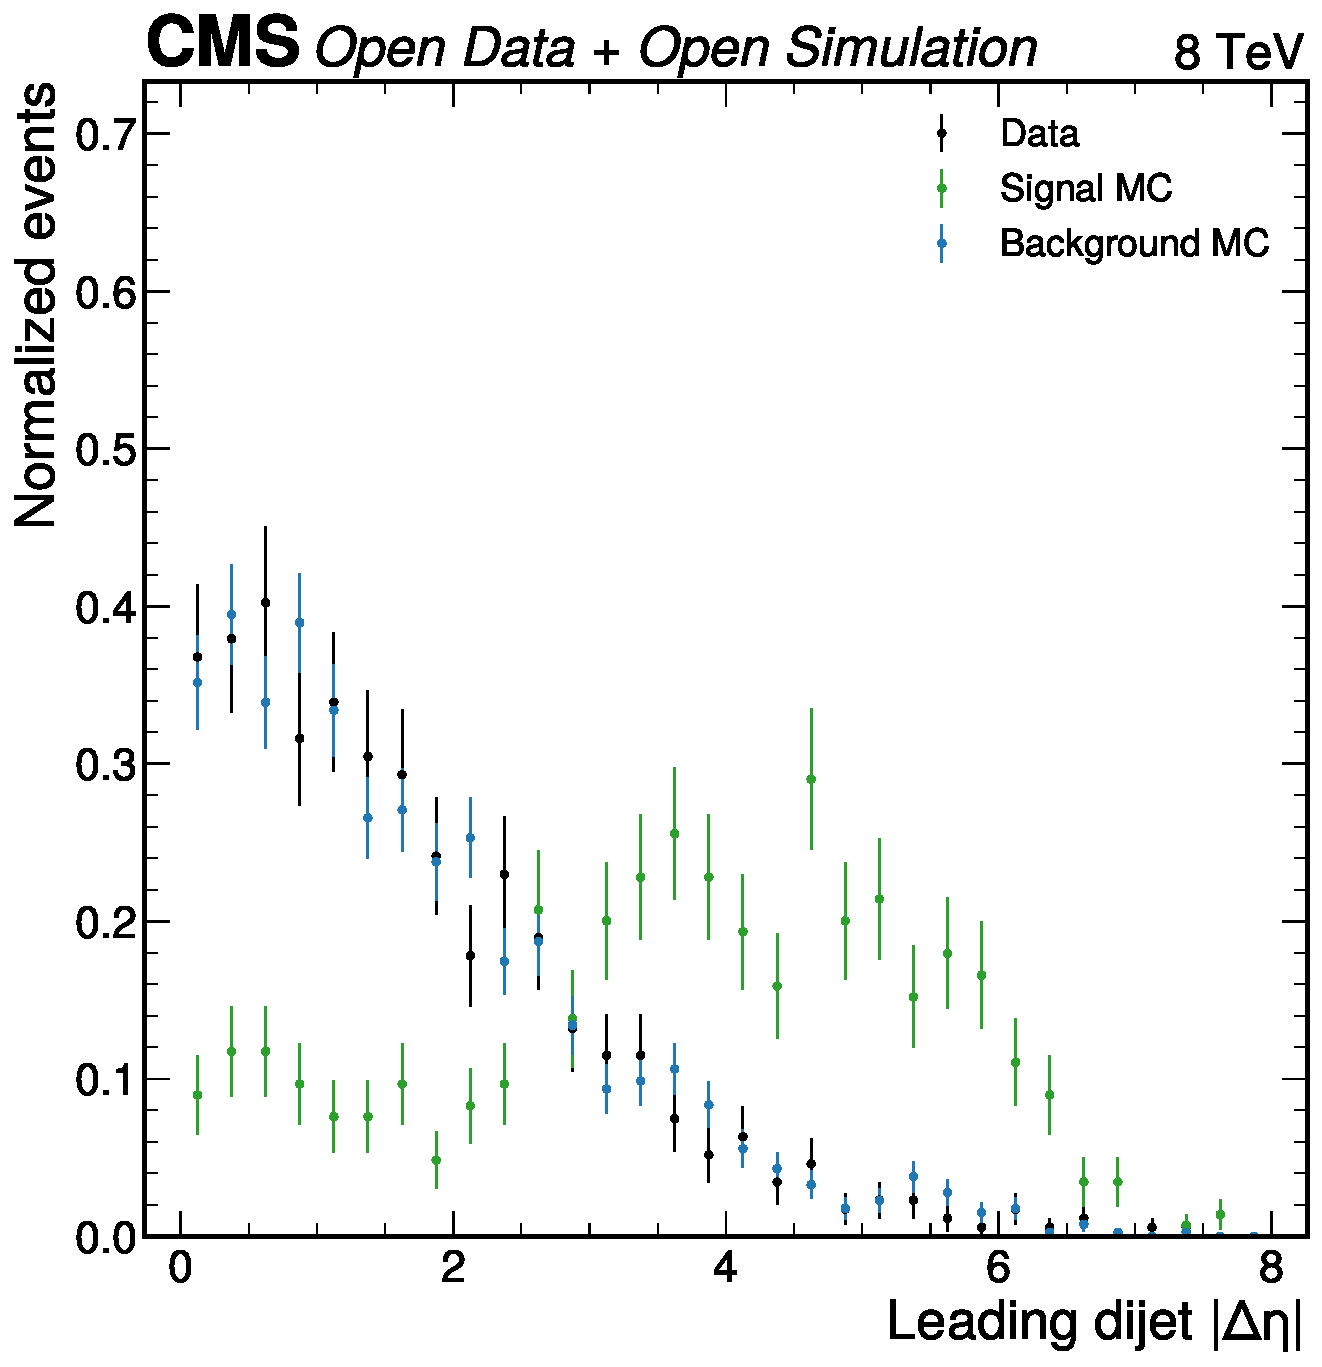
\includegraphics[height=0.35\textheight,width=\linewidth,keepaspectratio,alt={VBF dijet-rapidity-separation comparison. This figure checks the second VBF topology variable used in category assignment. Together with fig.~, it documents the topology basis for separating VBF from boosted and zero-jet events.}]{figures/vbf_delta_eta_jj.pdf}}
\caption{VBF dijet-rapidity-separation comparison. This figure checks
the second VBF topology variable used in category assignment. Together
with Figure~\ref{fig:app-vbf-mjj}, it documents the topology basis for
separating VBF from boosted and zero-jet
events.}\label{fig:app-vbf-deta}
\end{figure}

\needspace{0.4\textheight}
\begin{figure}[htbp]
\centering
\pandocbounded{
\includegraphics[height=0.35\textheight,width=\linewidth,keepaspectratio,alt={Visible transverse-momentum proxy comparison. This figure summarizes the reconstructed di-tau transverse-momentum proxy available in the reduced inputs. It is retained as a modelling cross-check, not as a final-fit observable.}]{figures/pt_tautau_proxy.pdf}}
\caption{Visible transverse-momentum proxy comparison. This figure
summarizes the reconstructed di-tau transverse-momentum proxy available
in the reduced inputs. It is retained as a modelling cross-check, not as
a final-fit observable.}\label{fig:app-pt-tautau}
\end{figure}

\needspace{0.4\textheight}
\begin{figure}[htbp]
\centering
\pandocbounded{
\includegraphics[height=0.35\textheight,width=\linewidth,keepaspectratio,alt={Z-rich visible-mass validation. This control-style figure checks the visible-mass shape in a Z-enriched region. The final note uses it as supporting evidence for the visible-mass baseline while keeping the DY/Z normalization uncertainty explicit.}]{figures/z_rich_validation_mvis.pdf}}
\caption{Z-rich visible-mass validation. This control-style figure
checks the visible-mass shape in a Z-enriched region. The final note
uses it as supporting evidence for the visible-mass baseline while
keeping the DY/Z normalization uncertainty
explicit.}\label{fig:app-z-rich}
\end{figure}

\needspace{0.4\textheight}
\begin{figure}[htbp]
\centering
\pandocbounded{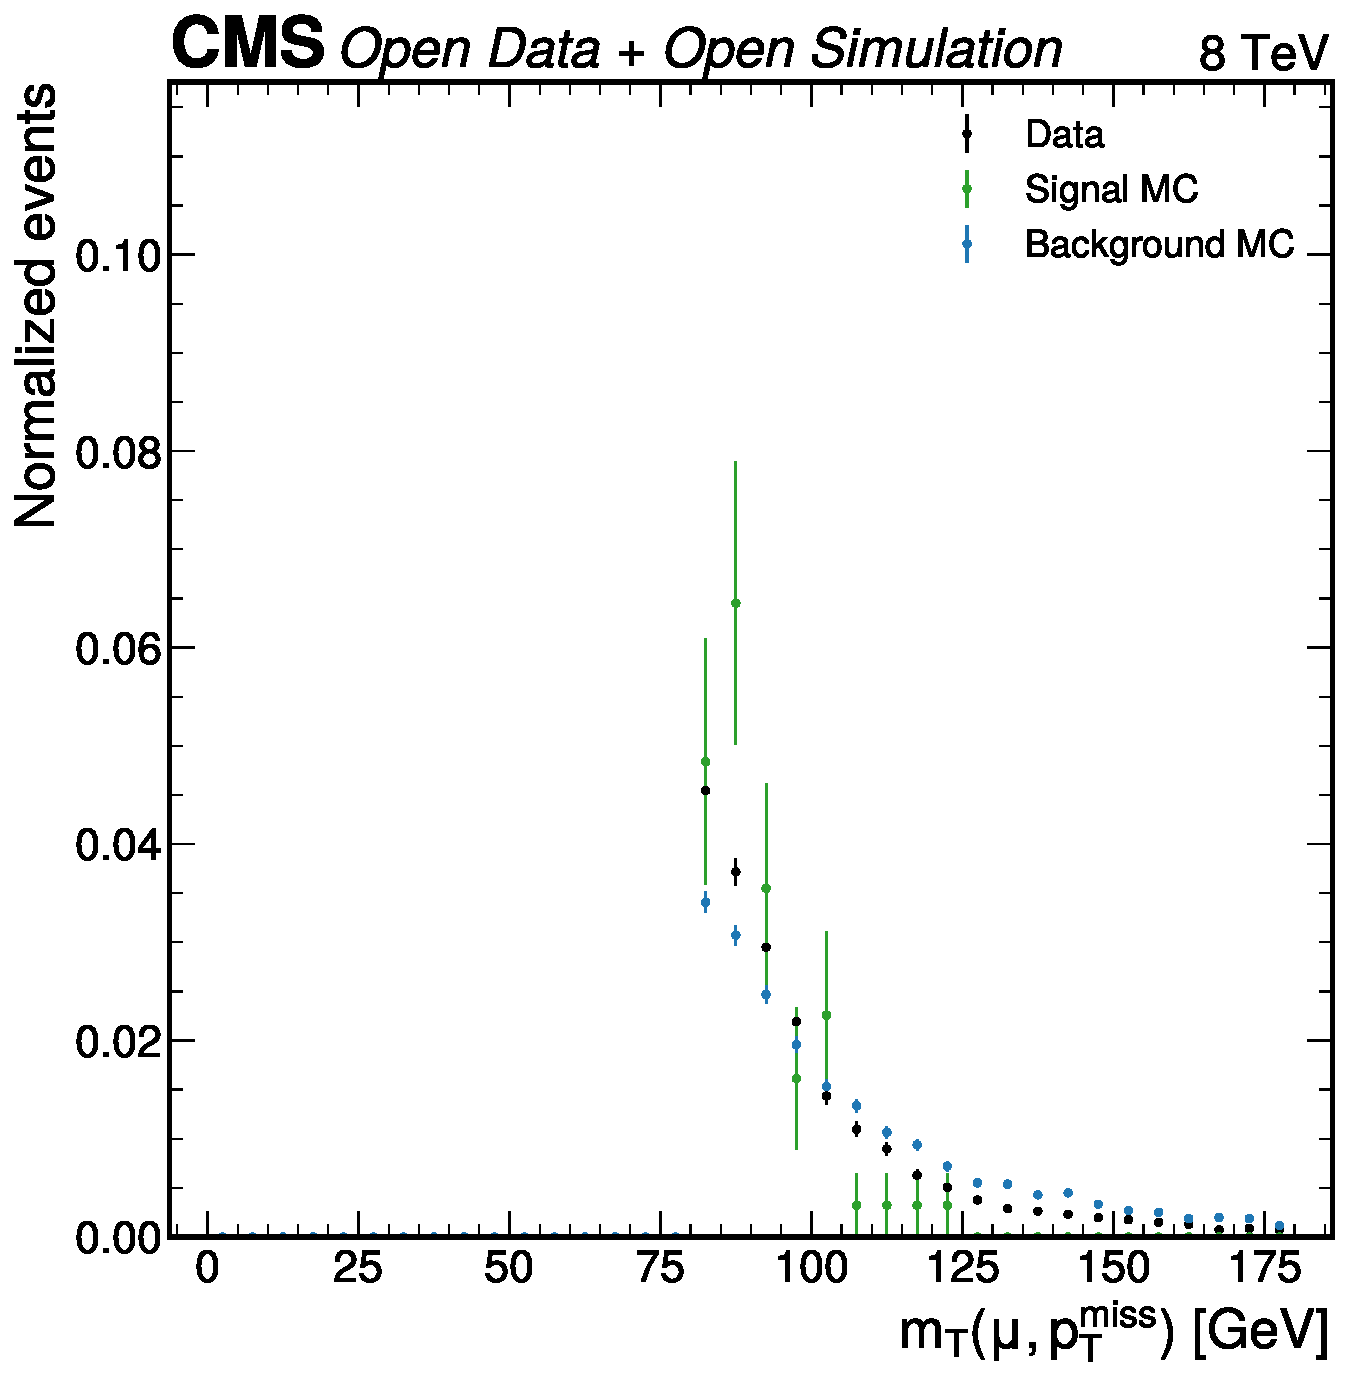
\includegraphics[height=0.35\textheight,width=\linewidth,keepaspectratio,alt={W high-mT control comparison. This figure shows the control-region distribution used for the W+jets normalization correction. It complements the numerical W scale in eq.~ by showing the region from which the scale is derived.}]{figures/w_high_mt_control_mt.pdf}}
\caption{W high-mT control comparison. This figure shows the
control-region distribution used for the W+jets normalization
correction. It complements the numerical W scale in Equation~\ref{eq:w-scale}
by showing the region from which the scale is
derived.}\label{fig:app-w-control}
\end{figure}

\needspace{0.4\textheight}
\begin{figure}[htbp]
\centering
\pandocbounded{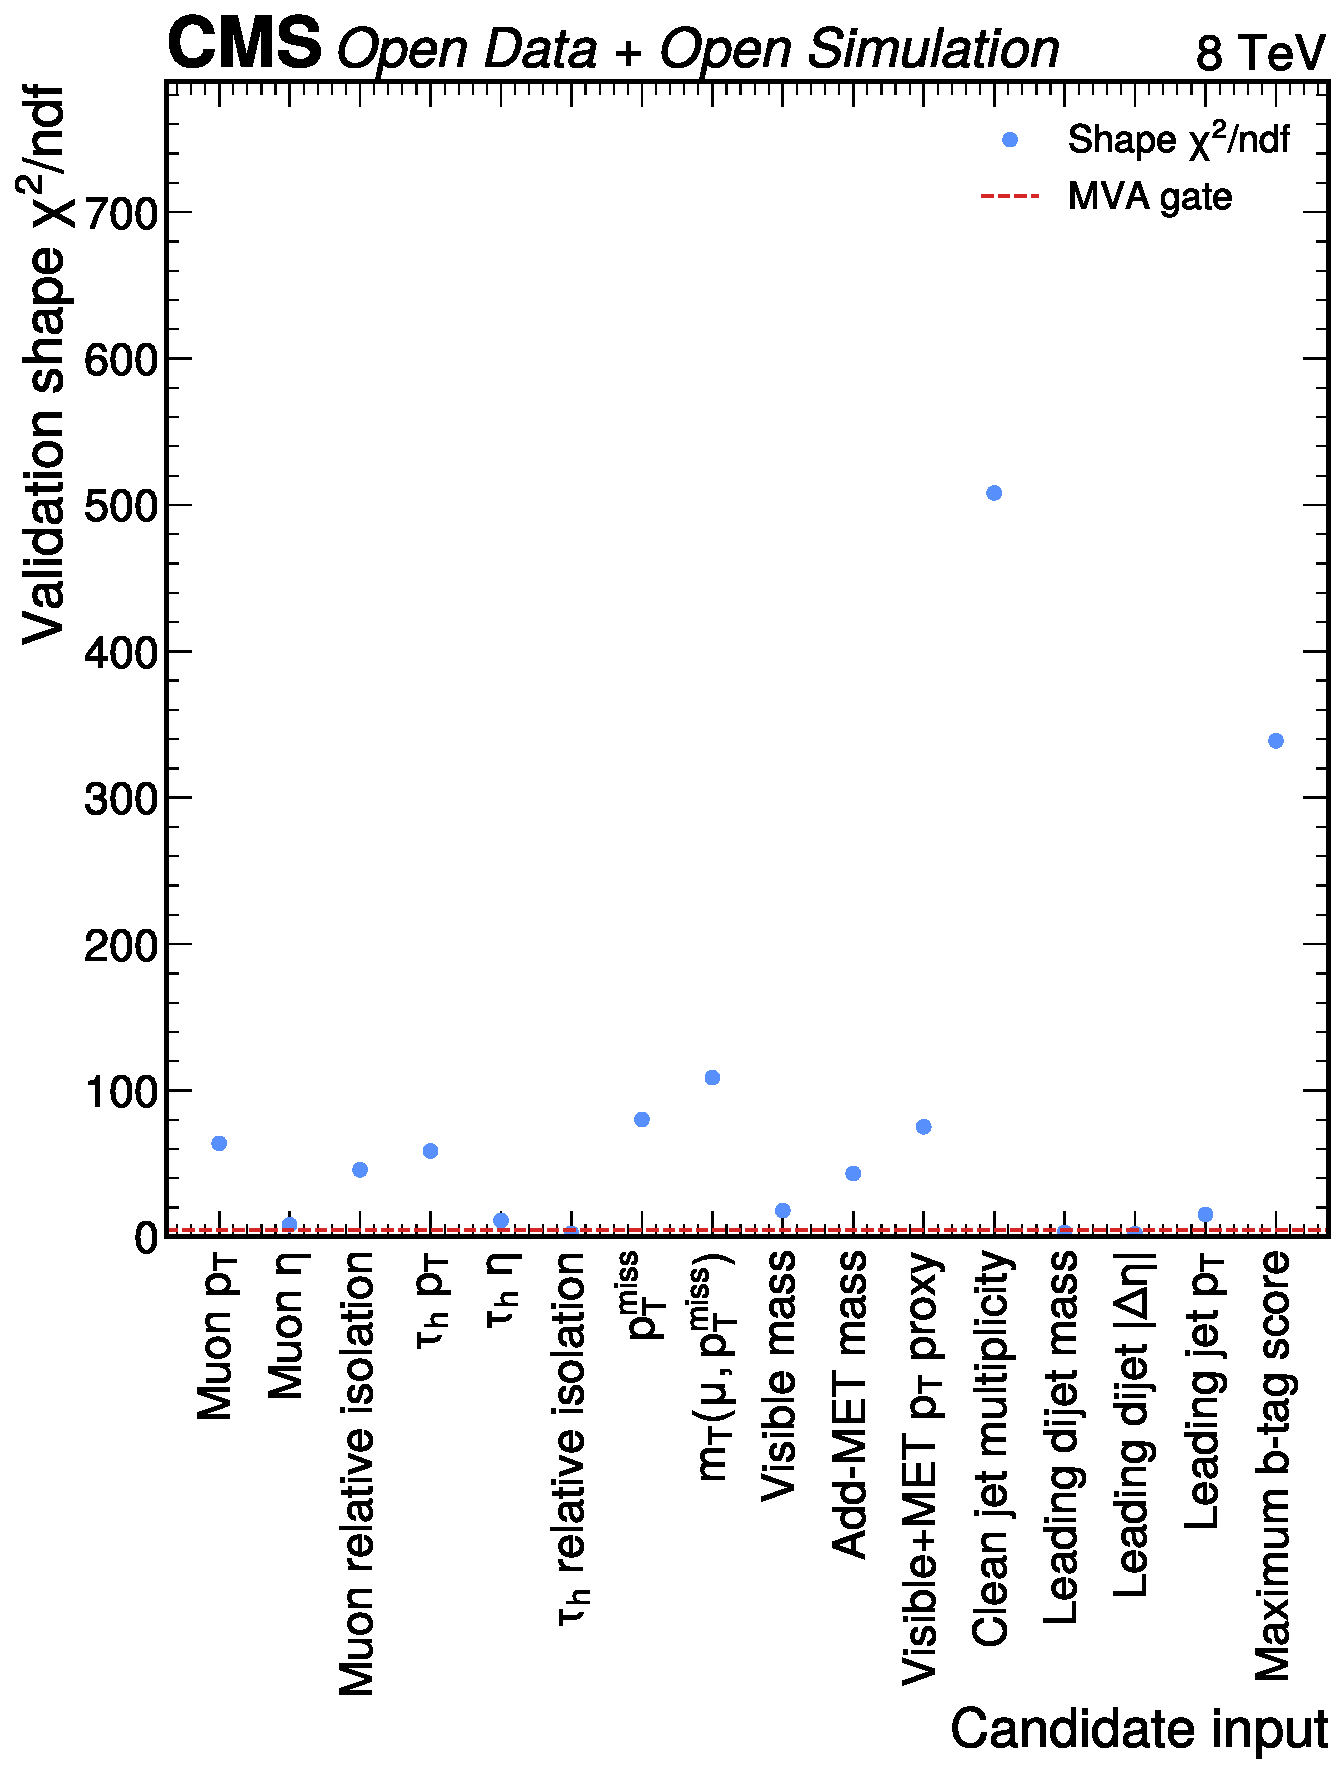
\includegraphics[height=0.35\textheight,width=\linewidth,keepaspectratio,alt={MVA input modelling summary. This figure records the input-modelling chi2 diagnostics that prevented an unqualified promotion of a classifier observable. It is included to make the rejected-classifier decision reproducible without reading the Phase 3 code.}]{figures/mva_input_modeling_chi2.pdf}}
\caption{MVA input modelling summary. This figure records the
input-modelling chi2 diagnostics that prevented an unqualified promotion
of a classifier observable. It is included to make the
rejected-classifier decision reproducible without reading the Phase 3
code.}\label{fig:app-mva-input}
\end{figure}

\needspace{0.4\textheight}
\begin{figure}[htbp]
\centering
\pandocbounded{
\includegraphics[height=0.35\textheight,width=\linewidth,keepaspectratio,alt={Expected signal-over-background summary. This expected-stage diagnostic shows why alternative observables were worth studying: the classifier and category choices can improve expected separation. The observed-data validation failure, not the expected-only sensitivity, determines the final model role.}]{figures/expected_s_over_b.pdf}}
\caption{Expected signal-over-background summary. This expected-stage
diagnostic shows why alternative observables were worth studying: the
classifier and category choices can improve expected separation. The
observed-data validation failure, not the expected-only sensitivity,
determines the final model role.}\label{fig:app-expected-sb}
\end{figure}

\needspace{0.4\textheight}
\begin{figure}[htbp]
\centering
\pandocbounded{
\includegraphics[height=0.35\textheight,width=\linewidth,keepaspectratio,alt={Approach comparison summary. This figure compares the broad observable strategies considered in the analysis chain. It documents that the final visible-mass result is a validation-driven choice rather than the most aggressive expected-sensitivity option.}]{figures/approach_comparison.pdf}}
\caption{Approach comparison summary. This figure compares the broad
observable strategies considered in the analysis chain. It documents
that the final visible-mass result is a validation-driven choice rather
than the most aggressive expected-sensitivity
option.}\label{fig:app-approach}
\end{figure}
\clearpage

\needspace{4\baselineskip}
\section*{References}\label{references}
\addcontentsline{toc}{section}{References}

\protect\phantomsection\label{refs}
\begin{CSLReferences}{1}{1}
\bibitem[\citeproctext]{ref-atlas_cms_higgs_combination_2016}
ATLAS and CMS Collaborations. 2016. {``Measurements of the Higgs Boson
Production and Decay Rates and Constraints on Its Couplings from a
Combined ATLAS and CMS Analysis of the LHC Pp Collision Data at Sqrt s =
7 and 8 TeV.''} \emph{Journal of High Energy Physics} 2016 (8): 45.
\url{https://doi.org/10.1007/JHEP08(2016)045}.

\bibitem[\citeproctext]{ref-cms_htt_2014}
CMS Collaboration. 2014. {``Evidence for the 125 GeV Higgs Boson
Decaying to a Pair of Tau Leptons.''} \emph{Journal of High Energy
Physics} 2014 (5): 104. \url{https://doi.org/10.1007/JHEP05(2014)104}.

\bibitem[\citeproctext]{ref-cms_htt_2018}
CMS Collaboration. 2018. {``Observation of the SM Scalar Boson Decaying
to a Pair of Tau Leptons with the CMS Experiment at the LHC.''}
\emph{Physics Letters B} 779: 283--316.
\url{https://doi.org/10.1016/j.physletb.2018.02.004}.

\bibitem[\citeproctext]{ref-cms_open_data_skim}
CMS Open Data Analyses. 2021. \emph{HiggsTauTauNanoAODOutreachAnalysis
Skim Code}.
\url{https://github.com/cms-opendata-analyses/HiggsTauTauNanoAODOutreachAnalysis}.

\bibitem[\citeproctext]{ref-cowan_asymptotic}
Cowan, Glen, Kyle Cranmer, Eilam Gross, and Ofer Vitells. 2011.
{``Asymptotic Formulae for Likelihood-Based Tests of New Physics.''}
\emph{European Physical Journal C} 71: 1554.
\url{https://doi.org/10.1140/epjc/s10052-011-1554-0}.

\bibitem[\citeproctext]{ref-pyhf_joss}
Heinrich, Lukas, Matthew Feickert, Giordon Stark, and Kyle Cranmer.
2021. {``Pyhf: Pure-Python Implementation of HistFactory Statistical
Models.''} \emph{Journal of Open Source Software} 6 (58): 2823.
\url{https://doi.org/10.21105/joss.02823}.

\bibitem[\citeproctext]{ref-lhc_hxswg_yellow_report_4}
LHC Higgs Cross Section Working Group. 2017. \emph{Handbook of LHC Higgs
Cross Sections: 4. Deciphering the Nature of the Higgs Sector}. CERN.
\url{https://doi.org/10.23731/CYRM-2017-002}.

\bibitem[\citeproctext]{ref-pdg_higgs_status_2024}
Particle Data Group. 2024. \emph{Status of Higgs Boson Physics}. Review
article in the 2024 Review of Particle Physics.
\url{https://pdg.lbl.gov/2024/reviews/rpp2024-rev-higgs-boson.pdf}.

\bibitem[\citeproctext]{ref-read_cls}
Read, A. L. 2002. {``Presentation of Search Results: The CLs
Technique.''} \emph{Journal of Physics G} 28: 2693--704.
\url{https://doi.org/10.1088/0954-3899/28/10/313}.

\bibitem[\citeproctext]{ref-cms_open_data_htt_2012}
Wunsch, Stefan. 2019. \emph{HiggsTauTauReduced: CMS Open Data Reduced
Samples for h to Tau Tau Studies}.
\url{https://doi.org/10.7483/OPENDATA.CMS.GV20.PR5T}.

\end{CSLReferences}

\end{document}
